\documentclass[11pt,a4paper]{article}

\usepackage[spanish,es-tabla,es-noquoting]{babel}
\usepackage[utf8]{inputenc}
\usepackage[T1]{fontenc}
\usepackage[top=2.5cm,bottom=3cm,left=2.5cm,right=2.5cm,headheight=75pt]{geometry}
\usepackage{amsmath,amssymb}
\usepackage{graphicx}
\usepackage[colorlinks=true, linkcolor=blue, urlcolor=blue, citecolor=blue]{hyperref}
\usepackage{fancyhdr}
\usepackage{booktabs}
\usepackage{tabularx}
\usepackage{float}
\usepackage{listings}
\usepackage{xcolor}
\usepackage{caption}
\usepackage{subcaption}

% Configuración de encabezado y pie de página institucional
\pagestyle{fancy}
\fancyhf{}
\fancyhead[C]{%
    \begin{minipage}[c]{1.8cm}
        
\includegraphics[width=1.6cm]{imagenes/uta.png}
    \end{minipage}%
    \hfill
    \begin{minipage}[c]{12cm} 
        \centering
        \small {\textbf{UNIVERSIDAD TÉCNICA DE AMBATO}} \\[0.1cm]
        \scriptsize \textit{FACULTAD DE INGENIERÍA EN SISTEMAS, ELECTRÓNICA E INDUSTRIAL} \\[0.1cm]
        \scriptsize \textbf{CARRERA DE SOFTWARE --- APLICACIONES ORIENTADAS A SERVICIOS} \\[0.1cm]
        \scriptsize \textbf{TALLER PRÁCTICO INDIVIDUAL: 20 RETOS DE SERVICIOS REST INTEGRADOS}
    \end{minipage}%
    \hfill
    \begin{minipage}[c]{1.8cm}
        \centering
        
\includegraphics[width=1.6cm]{imagenes/fisei.png}
    \end{minipage}%
}
\fancyfoot[C]{\thepage}
\renewcommand{\headrulewidth}{0.8pt}
\renewcommand{\footrulewidth}{0.4pt}

% Configuración de listados de código
\definecolor{codegreen}{rgb}{0,0.6,0}
\definecolor{codegray}{rgb}{0.5,0.5,0.5}
\definecolor{codepurple}{rgb}{0.58,0,0.82}
\definecolor{backcolour}{rgb}{0.96,0.97,0.98}

\lstdefinestyle{mystyle}{
    backgroundcolor=\color{backcolour},   
    commentstyle=\color{codegreen},
    keywordstyle=\color{blue}\bfseries,
    numberstyle=\tiny\color{codegray},
    stringstyle=\color{codepurple},
    basicstyle=\ttfamily\footnotesize,
    breakatwhitespace=false,         
    breaklines=true,                 
    captionpos=b,                    
    keepspaces=true,                 
    numbers=left,                    
    numbersep=5pt,                  
    showspaces=false,                
    showstringspaces=false,
    showtabs=false,                  
    tabsize=2,
    frame=single,
    rulecolor=\color{black!20},
    extendedchars=true,
    literate=
      {á}{{\'a}}1
      {é}{{\'e}}1
      {í}{{\'i}}1
      {ó}{{\'o}}1
      {ú}{{\'u}}1
      {Á}{{\'A}}1
      {É}{{\'E}}1
      {Í}{{\'I}}1
      {Ó}{{\'O}}1
      {Ú}{{\'U}}1
      {ñ}{{\~n}}1
      {Ñ}{{\~N}}1
}
\lstset{style=mystyle}

\begin{document}

% ============================================================================
% PORTADA
% ============================================================================
\begin{titlepage}
    \centering
    \vspace*{0.5cm}
    {\Large \textbf{UNIVERSIDAD TÉCNICA DE AMBATO}}\\[0.2cm]
    {\large \textbf{FACULTAD DE INGENIERÍA EN SISTEMAS, ELECTRÓNICA E INDUSTRIAL}}\\[0.2cm]
    {\textbf{CARRERA DE SOFTWARE}}\\[1.5cm]

    
\includegraphics[width=4cm]{imagenes/uta.png}\\[1.5cm]

    {\LARGE \textbf{INFORME TÉCNICO DE IMPLEMENTACIÓN}}\\[0.4cm]
    {\large \textbf{TALLER PRÁCTICO: RETOS DE SERVICIOS REST INTEGRADOS}}\\[0.2cm]
    {\textbf{Nivel 1 (F01 a F05) y Nivel 2 (D06 a D10)}}\\[1.5cm]

    \begin{flushleft}
    \begin{tabular}{ll}
        \textbf{Asignatura:} & Aplicaciones Orientadas a Servicios (SOA) \\
        \textbf{Ciclo / Nivel:} & Quinto Semestre --- Paralelo B \\
        \textbf{Estudiante:} & Molina Nuñez Karen Valeria \\
        \textbf{Docente:} & Ing. Javier Santiago Vargas Paredes, Mg. \\
        \textbf{Fecha de Entrega:} & Noviembre 2026 \\
        \textbf{Repositorio:} & Sistema Integrado Python (FastAPI) + Java (Spring Boot) + MySQL \\
    \end{tabular}
    \end{flushleft}

    \vfill
    {\small Ambato --- Ecuador}
\end{titlepage}

\newpage
\tableofcontents
\newpage

% ============================================================================
% 1. INTRODUCCIÓN Y ARQUITECTURA
% ============================================================================
\section{Introducción y Arquitectura del Sistema}

El presente documento detalla el diagnóstico, diseño técnico, implementación y validación experimental de los diez primeros retos prácticos correspondientes al \textbf{Nivel 1 · Retos Fáciles (F01 a F05)} y \textbf{Nivel 2 · Retos Difíciles (D06 a D10)} del sistema distribuido de vehículos y ventas.

La arquitectura del sistema está compuesta por los siguientes servicios desacoplados:
\begin{itemize}
    \item \textbf{Servicio de Ventas (\texttt{ventas-api}):} Microservicio desarrollado en Python utilizando FastAPI (puerto \texttt{8000}), SQLAlchemy como ORM, migraciones automáticas con Alembic y validación estricta de esquemas mediante Pydantic.
    \item \textbf{Servicio Central de Vehículos y Seguridad (\texttt{venta-vehiculos-api\_security}):} Servicio desarrollado en Java con Spring Boot (puerto \texttt{8081}), Spring Security y JPA/Hibernate para el catálogo de vehículos, emisión y validación de tokens OAuth2/JWT y gestión de reservas.
    \item \textbf{Base de Datos (\texttt{MySQL / XAMPP}):} Instancia relacional en el puerto \texttt{3306} (\texttt{venta\_vehiculos}), con integridad referencial compartida entre las tablas de Java (\texttt{vehiculos}, \texttt{reservas}, \texttt{usuarios\_api}) y Python (\texttt{compradores}, \texttt{ventas}).
\end{itemize}

\subsection{Estructura en Capas del Proyecto}
Para cumplir estrictamente con los principios de diseño de software y separación de responsabilidades:
\begin{enumerate}
    \item \textbf{Capa de Controladores/Routers (\texttt{app/routers/ventas.py}, \texttt{VehiculoController.java}):} Atiende las peticiones HTTP entrantes, extrae y valida los parámetros de entrada mediante DTOs, inyecta la seguridad (JWT y verificación de roles/propiedad) y mapea las respuestas con los códigos de estado adecuados.
    \item \textbf{Capa de Servicio (\texttt{app/services/venta\_service.py}, \texttt{VehiculoService.java}):} Contiene las reglas de negocio, control de estados válidos, coordinación de llamadas remotas y transaccionalidad.
    \item \textbf{Capa de Repositorio / Persistencia (\texttt{VentaRepository}, \texttt{CompradorRepository}, \texttt{VehiculoRepository}):} Encargada exclusivamente del acceso a datos, ordenamiento determinista y consultas parametrizadas contra MySQL.
\end{enumerate}

\subsection{Autenticación Centralizada (Paso Previo)}
Todas las operaciones protegidas requieren un token Bearer emitido por el servicio Java mediante el endpoint \texttt{POST /oauth/token} con credenciales de cliente Basic Auth y grant type \texttt{password}. En la Figura~\ref{fig:login_admin} se evidencia la generación del token JWT para el usuario administrador \texttt{admin-local}.

\begin{figure}[H]
    \centering
    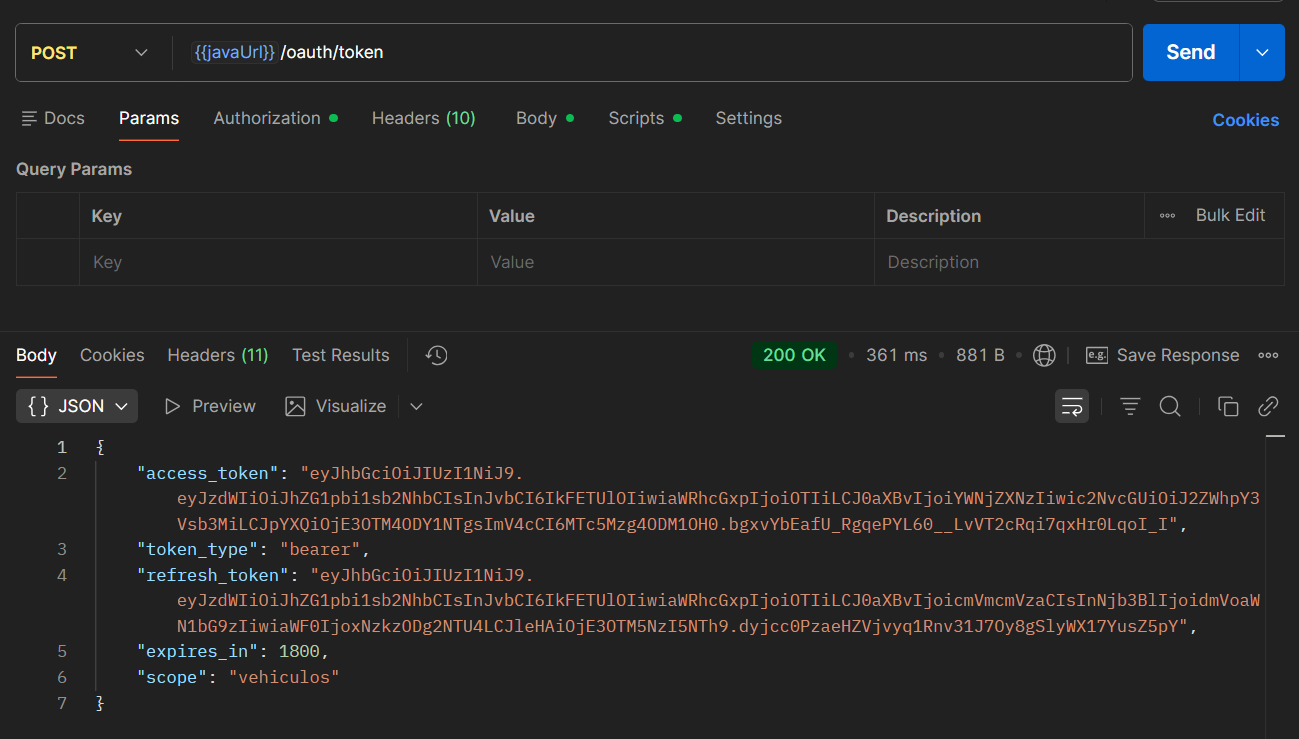
\includegraphics[width=0.95\textwidth]{imagenes/media/image1.png}
    \caption{Obtención del token JWT de autenticación mediante \texttt{POST /oauth/token} (200 OK).}
    \label{fig:login_admin}
\end{figure}

\newpage

% ============================================================================
% NIVEL 1 · RETOS FÁCILES (F01 - F05)
% ============================================================================
\section{Nivel 1 · Retos Fáciles (F01 a F05)}

% ----------------------------------------------------------------------------
% F01
% ----------------------------------------------------------------------------
\subsection{F01 | Listar compradores del usuario autenticado}
\textbf{Servicio y contrato:} FastAPI $\cdot$ \texttt{GET /api/compradores}

\subsubsection{1. Diagnóstico}
En el servicio base de \texttt{ventas-api} únicamente existía la operación \texttt{POST /api/compradores} para dar de alta registros. No se contaba con un endpoint para consultar la lista de compradores registrados por el vendedor autenticado, lo que impedía a los clientes frontend o móviles sincronizar su libreta de clientes.

\subsubsection{2. Diseño}
Se diseñó un endpoint \texttt{GET /api/compradores} protegido por la dependencia \texttt{identidad} y la política \texttt{vendedor(u)}, la cual exige roles \texttt{ROLE\_OPERADOR} o \texttt{ROLE\_ADMIN}. La consulta se filtra en SQLAlchemy de forma obligatoria por la columna \texttt{usuario = u["usuario"]}, garantizando aislamiento multi-inquilino. Si no hay compradores, responde una lista vacía \texttt{[]}.

\subsubsection{3. Implementación}
Se agregó el método \texttt{listar\_por\_usuario} en \texttt{CompradorRepository} y la ruta en \texttt{ventas.py}:
\begin{lstlisting}[language=Python]
@router.get("/compradores")
def listar_compradores(
    buscar: Annotated[str | None, Query()] = None,
    u=Depends(identidad)
):
    vendedor(u)
    with SessionLocal() as db:
        repo = CompradorRepository(db)
        compradores = repo.listar_por_usuario(u["usuario"], buscar=buscar)
        return [{"id": c.id, "documento": c.documento, "nombre": c.nombre, "correo": c.correo} for c in compradores]
\end{lstlisting}

\subsubsection{4. Validación}
\begin{table}[H]
\centering
\small
\begin{tabularx}{\textwidth}{l p{3.5cm} p{2.5cm} c c X}
\toprule
\textbf{ID} & \textbf{Método / URL} & \textbf{Condición / Auth} & \textbf{HTTP Esp.} & \textbf{HTTP Obt.} & \textbf{Resultado} \\
\midrule
F01-01 & \texttt{GET /api/compradores} & Token Bearer válido & 200 & 200 & Lista JSON con compradores propios. \\
F01-02 & \texttt{GET /api/compradores} & Sin cabecera Auth & 401 & 401 & Rechazo \texttt{NO\_AUTENTICADO}. \\
\bottomrule
\end{tabularx}
\caption{Matriz de pruebas del reto F01.}
\end{table}

\begin{figure}[H]
    \centering
    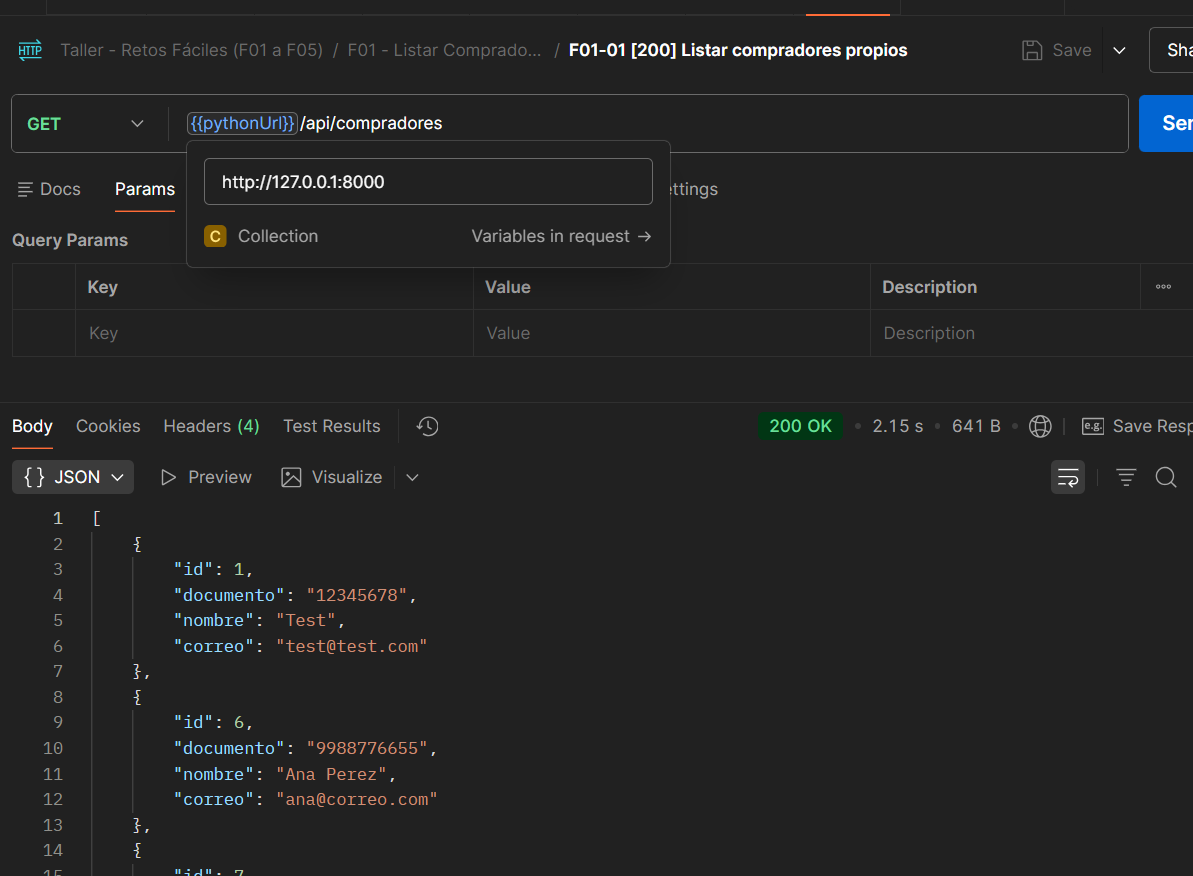
\includegraphics[width=0.95\textwidth]{imagenes/media/image2.png}
    \caption{F01-01: Listado propio exitoso (200 OK).}
    \label{fig:f01_01}
\end{figure}

\begin{figure}[H]
    \centering
    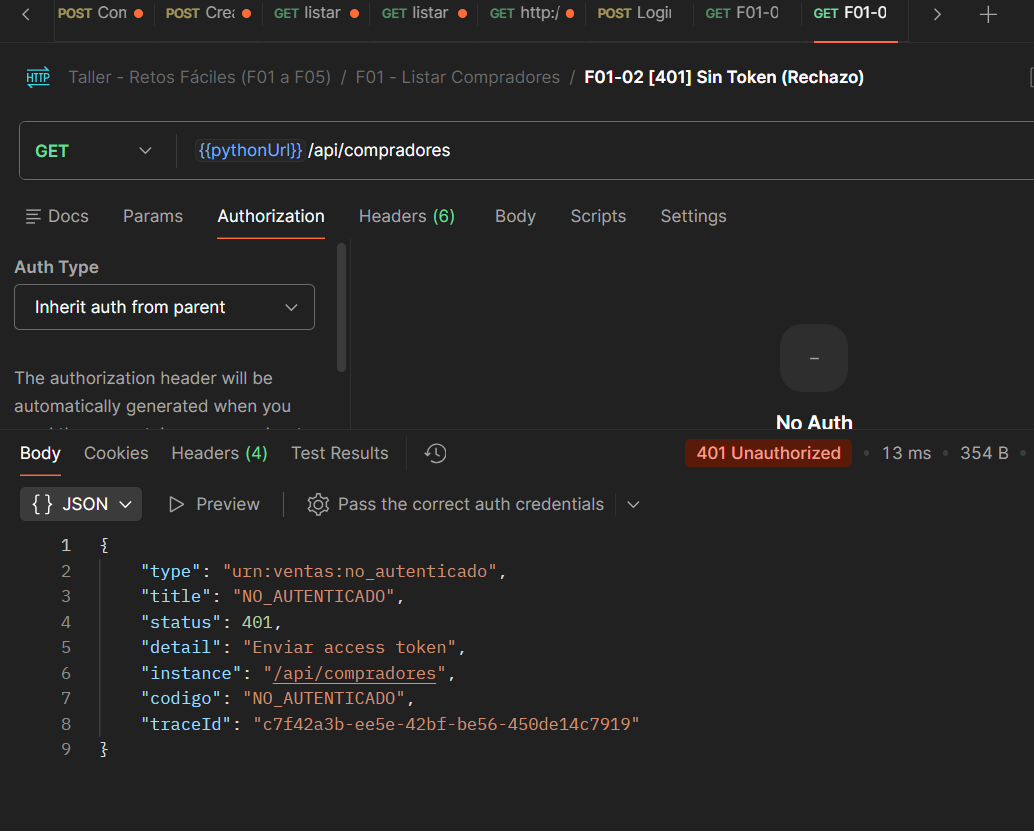
\includegraphics[width=0.95\textwidth]{imagenes/media/image3.png}
    \caption{F01-02: Rechazo sin token de autorización (401 Unauthorized).}
    \label{fig:f01_02}
\end{figure}

\subsubsection{5. Persistencia (MySQL)}
La consulta SQL ejecutada internamente es:
\begin{lstlisting}[language=SQL]
SELECT id, documento, nombre, correo, usuario FROM compradores WHERE usuario = 'admin-local';
\end{lstlisting}

\begin{figure}[H]
    \centering
    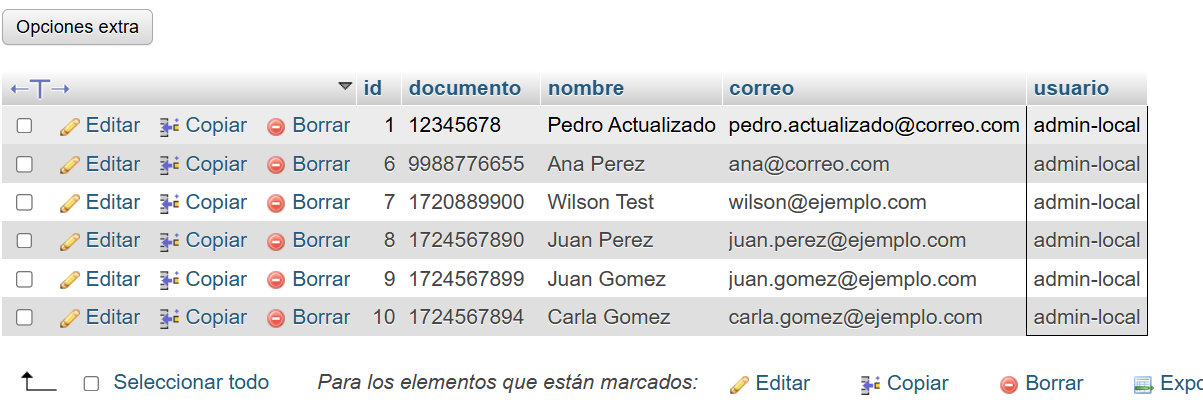
\includegraphics[width=0.95\textwidth]{imagenes/media/sql_f01_d07.png}
    \caption{Evidencia SQL en MySQL (phpMyAdmin) de compradores para el usuario admin-local.}
    \label{fig:sql_f01}
\end{figure}

\subsubsection{6. Explicación}
El filtrado reside en la capa Repository para aprovechar los índices de base de datos sobre \texttt{usuario}. La regla de seguridad se verifica en la capa Router antes de abrir la sesión de base de datos, optimizando recursos y garantizando que un usuario jamás acceda a compradores ajenos.

\newpage
% ----------------------------------------------------------------------------
% F02
% ----------------------------------------------------------------------------
\subsection{F02 | Consultar un comprador por identificador}
\textbf{Servicio y contrato:} FastAPI $\cdot$ \texttt{GET /api/compradores/\{id\}}

\subsubsection{1. Diagnóstico}
El sistema no permitía consultar el detalle de un comprador particular a partir de su clave primaria (\texttt{id}), imposibilitando verificar sus datos antes de asociarlo a una venta.

\subsubsection{2. Diseño}
Se diseñó la ruta parametrizada \texttt{GET /api/compradores/\{id\}}. Reglas aplicadas:
\begin{itemize}
    \item Si el registro no existe en MySQL, retornar \texttt{404 Not Found} con código \texttt{COMPRADOR\_NO\_EXISTE}.
    \item Si existe, validar con la función de seguridad \texttt{propietario(u, c.usuario)} que pertenezca al usuario o que este posea \texttt{ROLE\_ADMIN} (retornando \texttt{403} en caso contrario).
    \item Retornar únicamente atributos públicos: \texttt{id}, \texttt{documento}, \texttt{nombre}, \texttt{correo}.
\end{itemize}

\subsubsection{3. Implementación}
\begin{lstlisting}[language=Python]
@router.get("/compradores/{id}")
def obtener_comprador(id: int, u=Depends(identidad)):
    vendedor(u)
    with SessionLocal() as db:
        c = CompradorRepository(db).por_id(id)
        if c is None:
            raise ApiError(404, "COMPRADOR_NO_EXISTE", "Comprador inexistente")
        propietario(u, c.usuario)
        return {"id": c.id, "documento": c.documento, "nombre": c.nombre, "correo": c.correo}
\end{lstlisting}

\subsubsection{4. Validación}
\begin{table}[H]
\centering
\small
\begin{tabularx}{\textwidth}{l p{3.5cm} p{2.5cm} c c X}
\toprule
\textbf{ID} & \textbf{Método / URL} & \textbf{Condición / Auth} & \textbf{HTTP Esp.} & \textbf{HTTP Obt.} & \textbf{Resultado} \\
\midrule
F02-01 & \texttt{GET /api/compradores/1} & ID existente, propietario & 200 & 200 & Objeto JSON con datos del comprador. \\
F02-02 & \texttt{GET /api/compradores/99999} & ID inexistente & 404 & 404 & Rechazo \texttt{COMPRADOR\_NO\_EXISTE}. \\
\bottomrule
\end{tabularx}
\caption{Matriz de pruebas del reto F02.}
\end{table}

\begin{figure}[H]
    \centering
    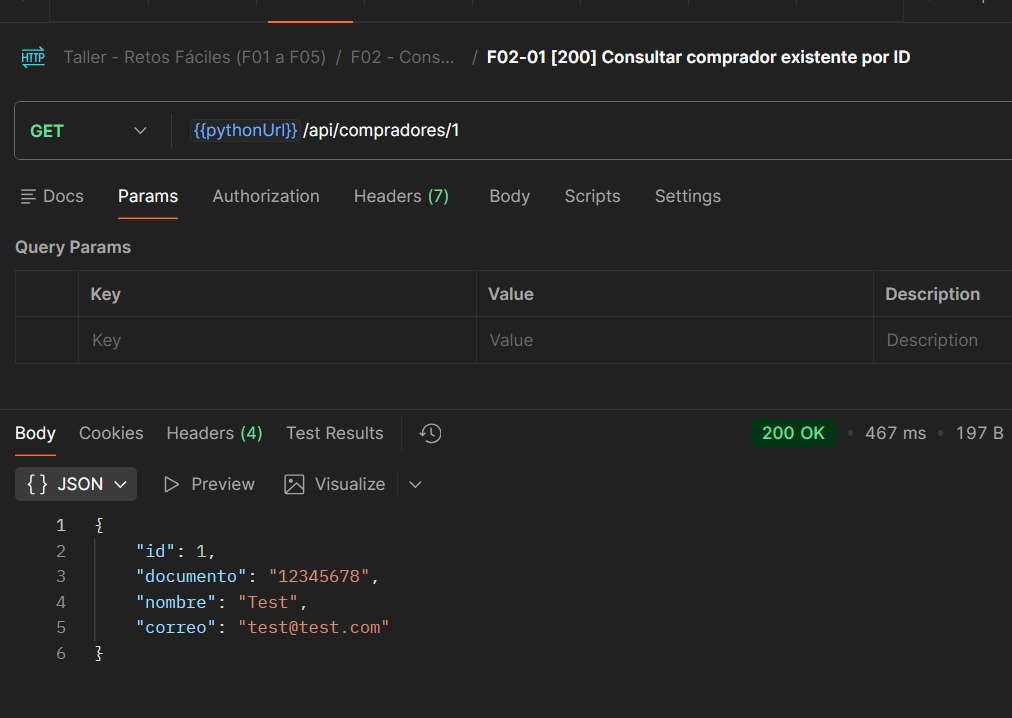
\includegraphics[width=0.95\textwidth]{imagenes/media/image4.png}
    \caption{F02-01: Consulta por ID exitosa (200 OK).}
    \label{fig:f02_01}
\end{figure}

\begin{figure}[H]
    \centering
    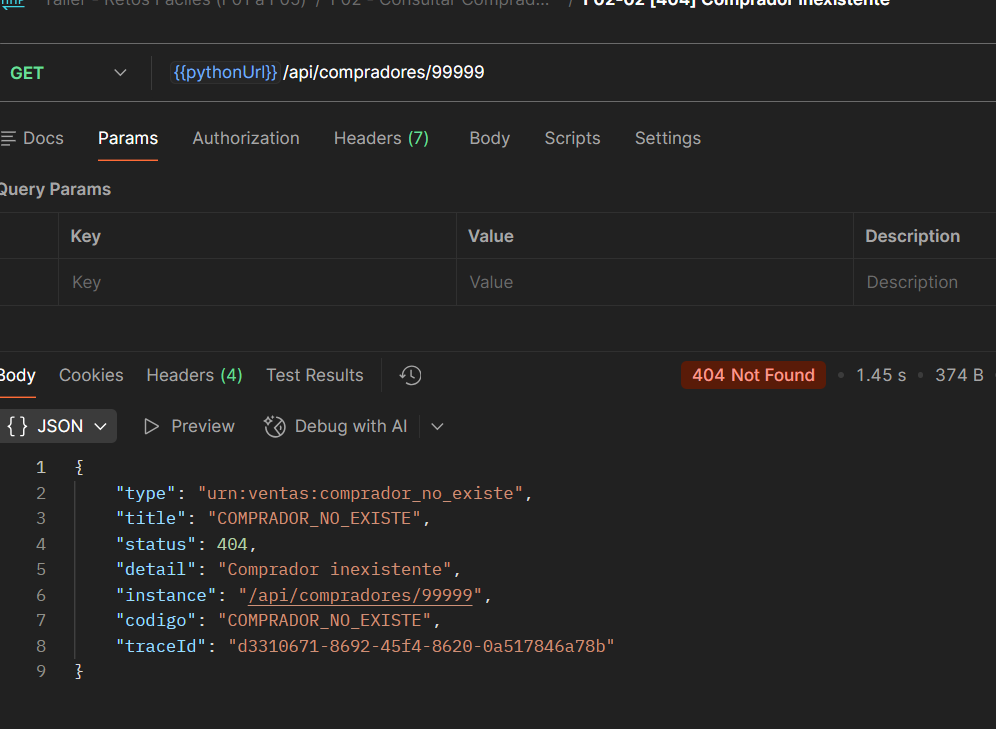
\includegraphics[width=0.95\textwidth]{imagenes/media/image5.png}
    \caption{F02-02: ID inexistente (404 Not Found).}
    \label{fig:f02_02}
\end{figure}

\subsubsection{5. Persistencia (MySQL)}
\begin{lstlisting}[language=SQL]
SELECT id, documento, nombre, correo, usuario FROM compradores WHERE id = 1;
\end{lstlisting}

\begin{figure}[H]
    \centering
    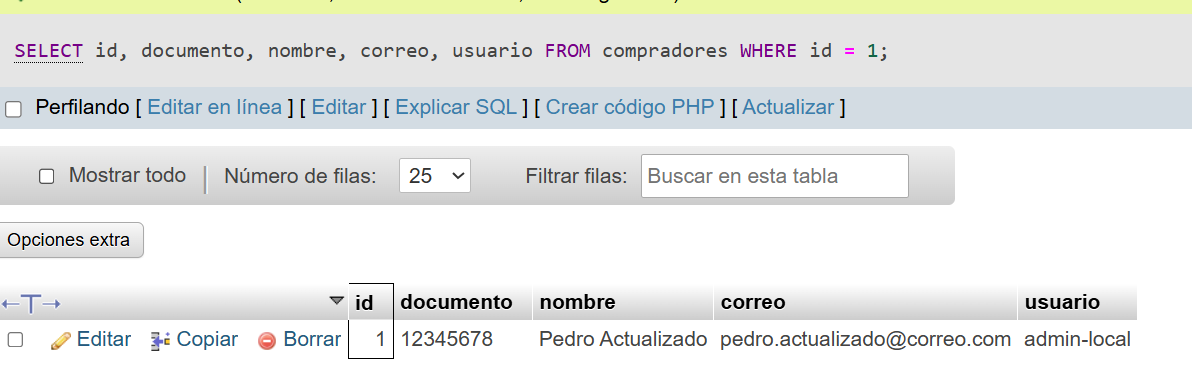
\includegraphics[width=0.95\textwidth]{imagenes/media/sql_f02_d08.png}
    \caption{Evidencia SQL en MySQL (phpMyAdmin) de la consulta individual del comprador ID 1.}
    \label{fig:sql_f02}
\end{figure}

\subsubsection{6. Explicación}
La verificación de existencia se ejecuta antes de la autorización para devolver códigos de error estándar conformes a RFC 7807 (Problem Details). La inmutabilidad de la información sensible interna se asegura al construir un DTO explícito de salida.

\newpage
% ----------------------------------------------------------------------------
% F03
% ----------------------------------------------------------------------------
\subsection{F03 | Listar ventas propias ordenadas}
\textbf{Servicio y contrato:} FastAPI $\cdot$ \texttt{GET /api/ventas}

\subsubsection{1. Diagnóstico}
La API de ventas disponía de consulta individual \texttt{GET /api/ventas/\{id\}}, pero carecía de una ruta raíz para listar el historial general de transacciones del usuario, dificultando el seguimiento de operaciones en curso.

\subsubsection{2. Diseño}
Se implementó el endpoint \texttt{GET /api/ventas} sin interferir con la ruta parametrizada por ID. Se estipuló un ordenamiento compuesto determinista: \texttt{fecha DESC, id DESC}, asegurando que las ventas más recientes encabecen la lista y garantizando estabilidad temporal cuando dos registros comparten la misma marca de tiempo.

\subsubsection{3. Implementación}
Se actualizó \texttt{VentaRepository.listar\_propias} con el ordenamiento requerido:
\begin{lstlisting}[language=Python]
def listar_propias(self, usuario: str, estado: str | None = None, limit: int | None = None, offset: int | None = None):
    stmt = select(Venta).where(Venta.usuario == usuario)
    if estado:
        stmt = stmt.where(Venta.estado == estado)
    stmt = stmt.order_by(Venta.fecha.desc(), Venta.id.desc())
    if limit is not None:
        stmt = stmt.limit(limit)
    if offset is not None:
        stmt = stmt.offset(offset)
    return self.db.scalars(stmt).all()
\end{lstlisting}

\subsubsection{4. Validación}
\begin{table}[H]
\centering
\small
\begin{tabularx}{\textwidth}{l p{3.5cm} p{2.5cm} c c X}
\toprule
\textbf{ID} & \textbf{Método / URL} & \textbf{Condición / Auth} & \textbf{HTTP Esp.} & \textbf{HTTP Obt.} & \textbf{Resultado} \\
\midrule
F03-01 & \texttt{GET /api/ventas} & Token válido & 200 & 200 & Listado de ventas ordenadas por fecha/ID descendente. \\
F03-02 & \texttt{GET /api/ventas} & Sin Token & 401 & 401 & Rechazo \texttt{NO\_AUTENTICADO}. \\
F03-03 & \texttt{GET /api/ventas/1} & Consulta puntual por ID & 200 & 200 & Objeto individual de la venta consultada. \\
\bottomrule
\end{tabularx}
\caption{Matriz de pruebas del reto F03.}
\end{table}

\begin{figure}[H]
    \centering
    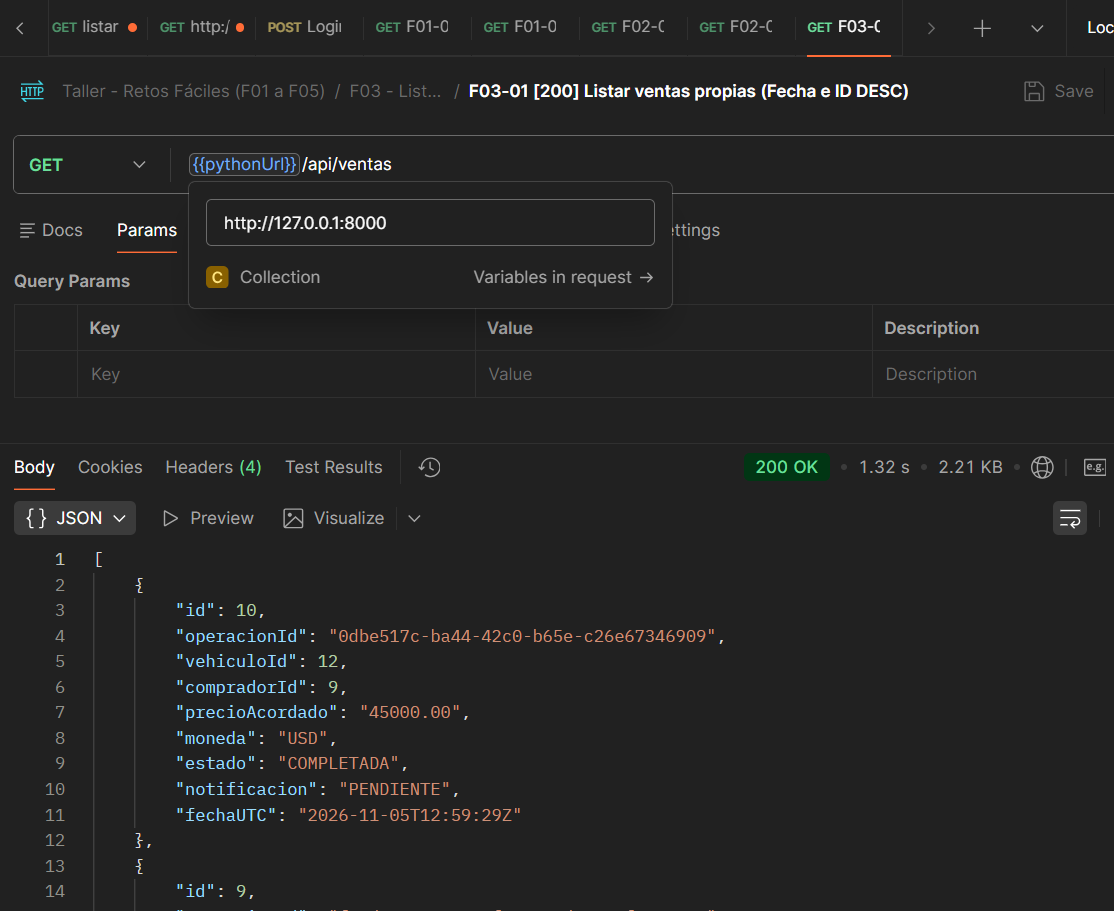
\includegraphics[width=0.95\textwidth]{imagenes/media/image6.png}
    \caption{F03-01: Listado ordenado por fecha e ID descendente (200 OK).}
    \label{fig:f03_01}
\end{figure}

\begin{figure}[H]
    \centering
    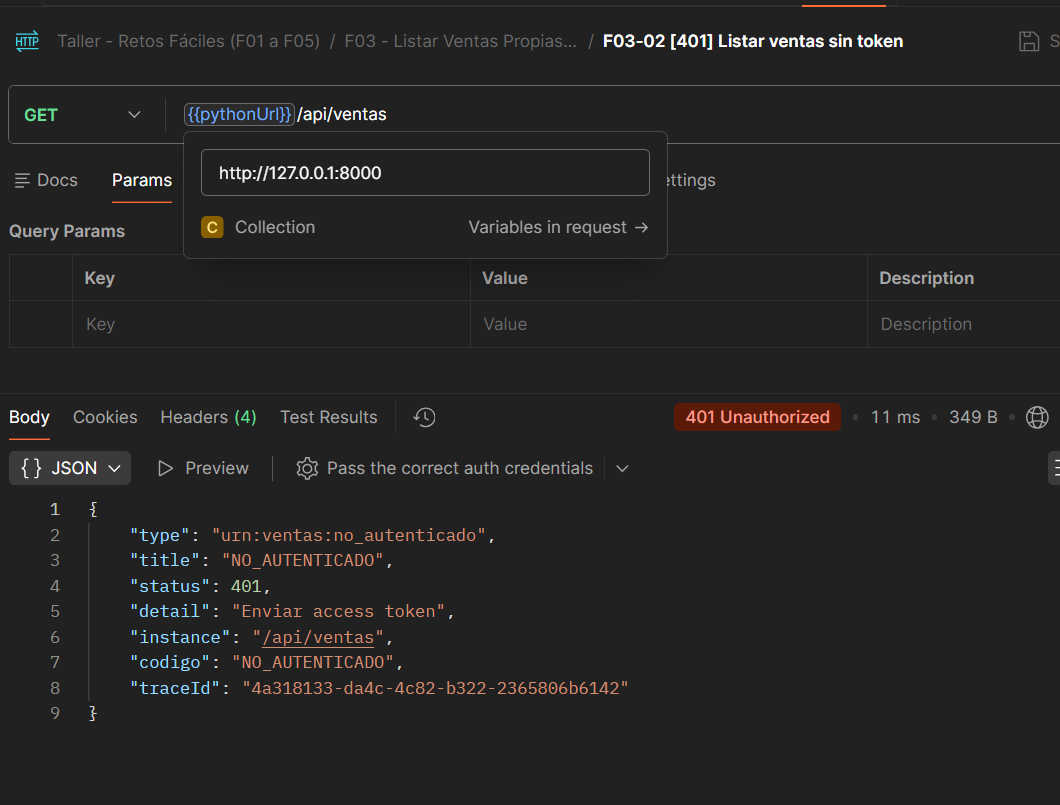
\includegraphics[width=0.95\textwidth]{imagenes/media/image7.png}
    \caption{F03-02: Rechazo sin token de autorización (401 Unauthorized).}
    \label{fig:f03_02}
\end{figure}

\begin{figure}[H]
    \centering
    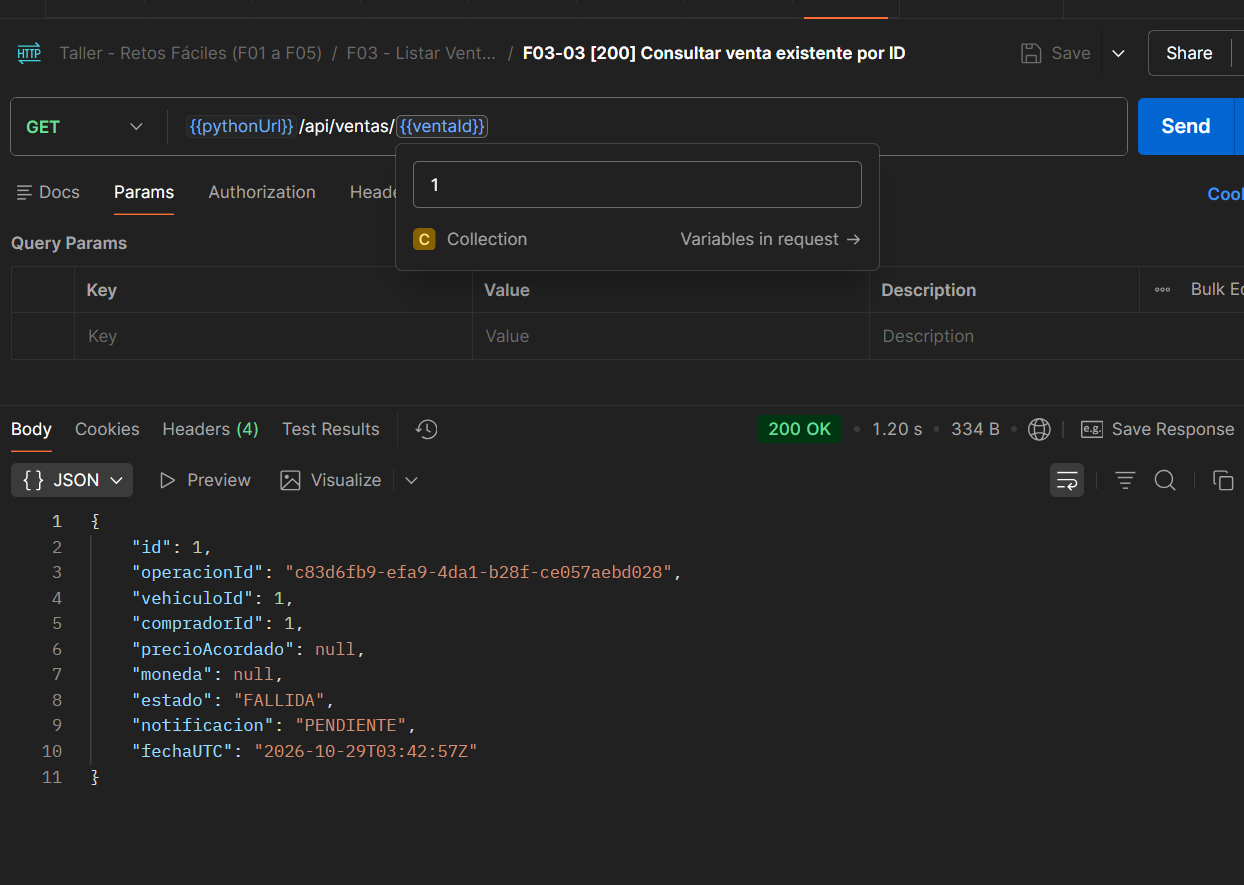
\includegraphics[width=0.95\textwidth]{imagenes/media/image8.png}
    \caption{F03-03: Consulta puntual de venta por ID existente (200 OK).}
    \label{fig:f03_03}
\end{figure}

\subsubsection{5. Persistencia (MySQL)}
\begin{lstlisting}[language=SQL]
SELECT id, operacion_id, vehiculo_id, comprador_id, estado, fecha 
FROM ventas WHERE usuario = 'admin-local' ORDER BY fecha DESC, id DESC;
\end{lstlisting}

\begin{figure}[H]
    \centering
    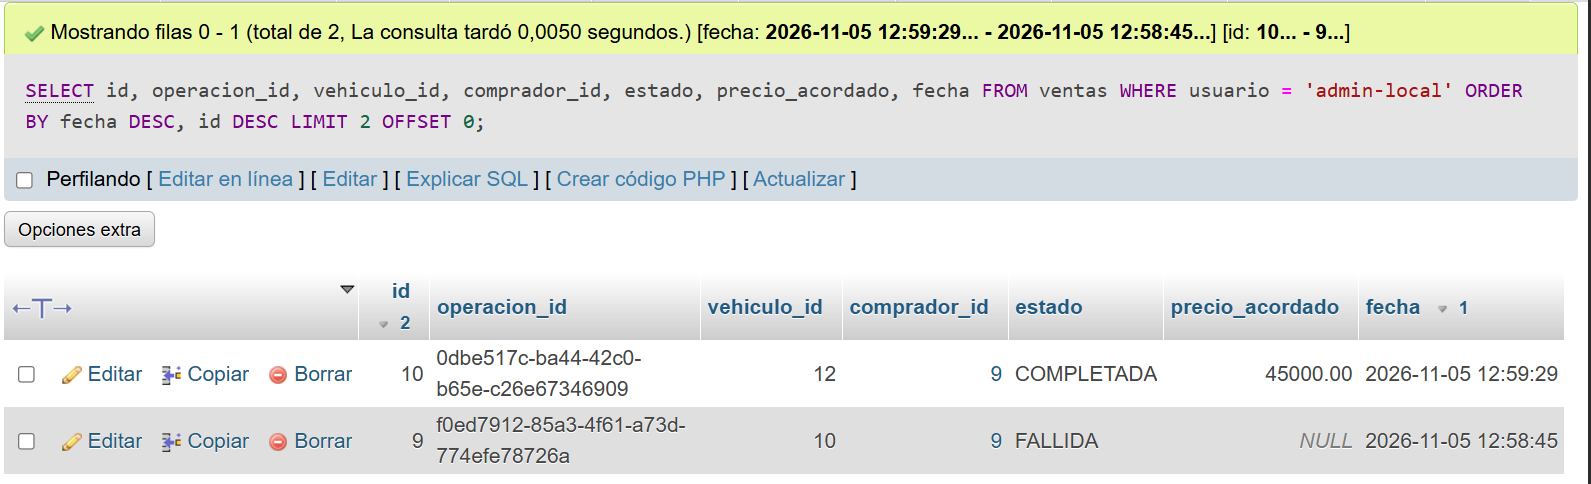
\includegraphics[width=0.95\textwidth]{imagenes/media/sql_f03_d06.png}
    \caption{Evidencia SQL en MySQL: Ventas ordenadas por fecha y ID descendente.}
    \label{fig:sql_f03}
\end{figure}

\subsubsection{6. Explicación}
El ordenamiento se realiza directamente en el motor relacional mediante \texttt{ORDER BY}, lo que permite al optimizador de MySQL utilizar índices primarios y de clave foránea, evitando ordenar colecciones en memoria de la aplicación.

\newpage
% ----------------------------------------------------------------------------
% F04
% ----------------------------------------------------------------------------
\subsection{F04 | Filtrar ventas por estado}
\textbf{Servicio y contrato:} FastAPI $\cdot$ \texttt{GET /api/ventas?estado=COMPLETADA}

\subsubsection{1. Diagnóstico}
El listado general de ventas mezclaba transacciones en cualquier estado, obligando a los clientes a procesar o filtrar listas extensas en el frontend para identificar ventas exitosas o fallidas.

\subsubsection{2. Diseño}
Se incorporó el parámetro de consulta opcional \texttt{estado}. Los estados admitidos corresponden al ciclo de vida formal del negocio: \texttt{PENDIENTE}, \texttt{EN\_REVISION}, \texttt{COMPLETADA} y \texttt{FALLIDA}. Cualquier valor no reconocido debe ser rechazado inmediatamente con error HTTP \texttt{422 Unprocessable Content} y código \texttt{ESTADO\_INVALIDO}.

\subsubsection{3. Implementación}
\begin{lstlisting}[language=Python]
ESTADOS_VENTA_VALIDOS = {"PENDIENTE", "EN_REVISION", "COMPLETADA", "FALLIDA"}

@router.get("/ventas")
def listar_ventas(estado: Annotated[str | None, Query()] = None, u=Depends(identidad)):
    vendedor(u)
    if estado is not None:
        estado_norm = estado.strip().upper()
        if estado_norm not in ESTADOS_VENTA_VALIDOS:
            raise ApiError(422, "ESTADO_INVALIDO", f"Valores admitidos: {sorted(ESTADOS_VENTA_VALIDOS)}")
        estado = estado_norm
    with SessionLocal() as db:
        ventas = VentaRepository(db).listar_propias(u["usuario"], estado=estado)
        return [service.salida(v) for v in ventas]
\end{lstlisting}

\subsubsection{4. Validación}
\begin{table}[H]
\centering
\small
\begin{tabularx}{\textwidth}{l p{4cm} p{2.5cm} c c X}
\toprule
\textbf{ID} & \textbf{Método / URL} & \textbf{Condición} & \textbf{HTTP Esp.} & \textbf{HTTP Obt.} & \textbf{Resultado} \\
\midrule
F04-01 & \texttt{GET /api/ventas?estado=COMPLETADA} & Estado válido & 200 & 200 & Solo ventas en estado COMPLETADA. \\
F04-02 & \texttt{GET /api/ventas?estado=FALLIDA} & Estado válido & 200 & 200 & Solo ventas en estado FALLIDA. \\
F04-03 & \texttt{GET /api/ventas?estado=EN\_REVISION} & Sin coincidencias & 200 & 200 & Lista vacía \texttt{[]}. \\
F04-04 & \texttt{GET /api/ventas?estado=ESTADO\_FALSO} & Estado no permitido & 422 & 422 & Rechazo controlado \texttt{ESTADO\_INVALIDO}. \\
\bottomrule
\end{tabularx}
\caption{Matriz de pruebas del reto F04.}
\end{table}

\begin{figure}[H]
    \centering
    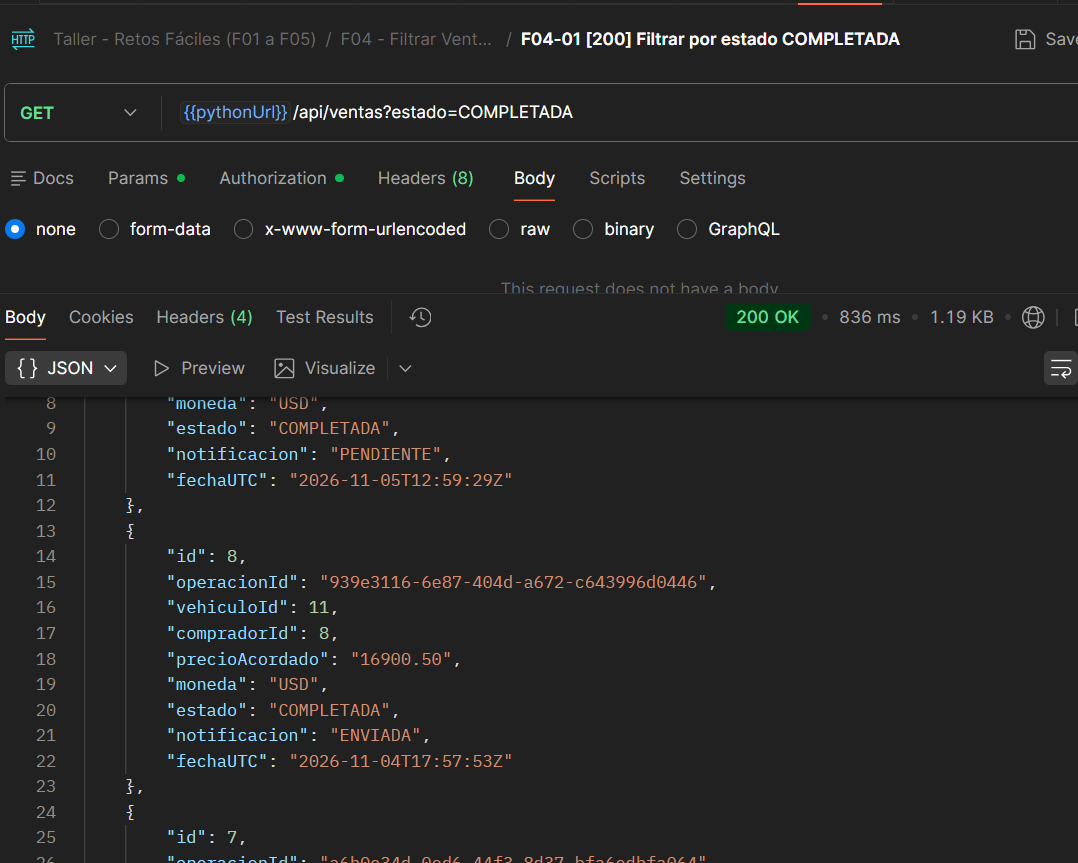
\includegraphics[width=0.95\textwidth]{imagenes/media/image9.png}
    \caption{F04-01: Filtro por estado COMPLETADA (200 OK).}
    \label{fig:f04_01}
\end{figure}

\begin{figure}[H]
    \centering
    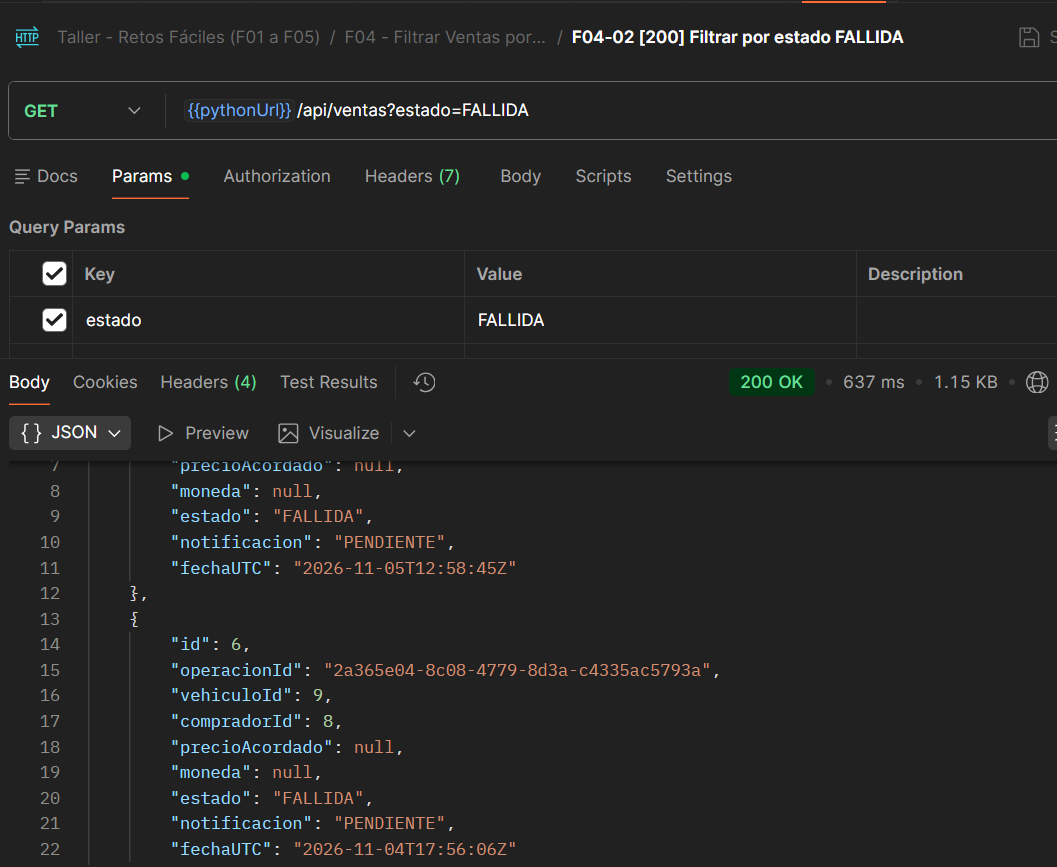
\includegraphics[width=0.95\textwidth]{imagenes/media/image10.png}
    \caption{F04-02: Filtro por estado FALLIDA (200 OK).}
    \label{fig:f04_02}
\end{figure}

\begin{figure}[H]
    \centering
    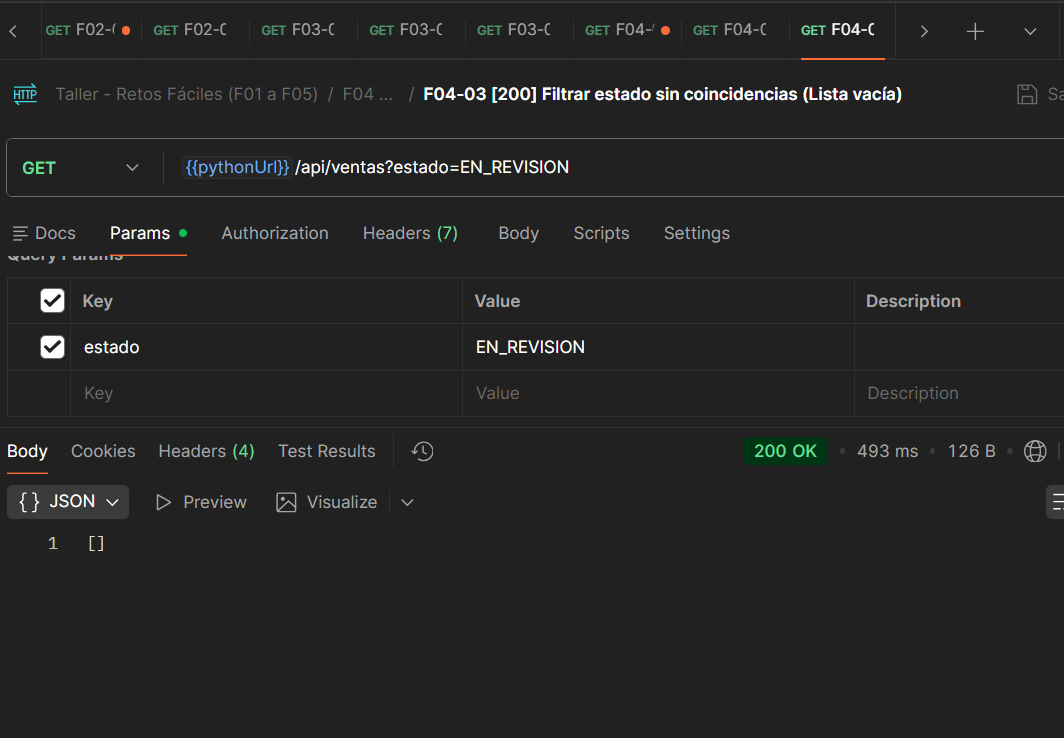
\includegraphics[width=0.95\textwidth]{imagenes/media/image11.png}
    \caption{F04-03: Filtro por estado EN\_REVISION sin coincidencias (200 OK []).}
    \label{fig:f04_03}
\end{figure}

\begin{figure}[H]
    \centering
    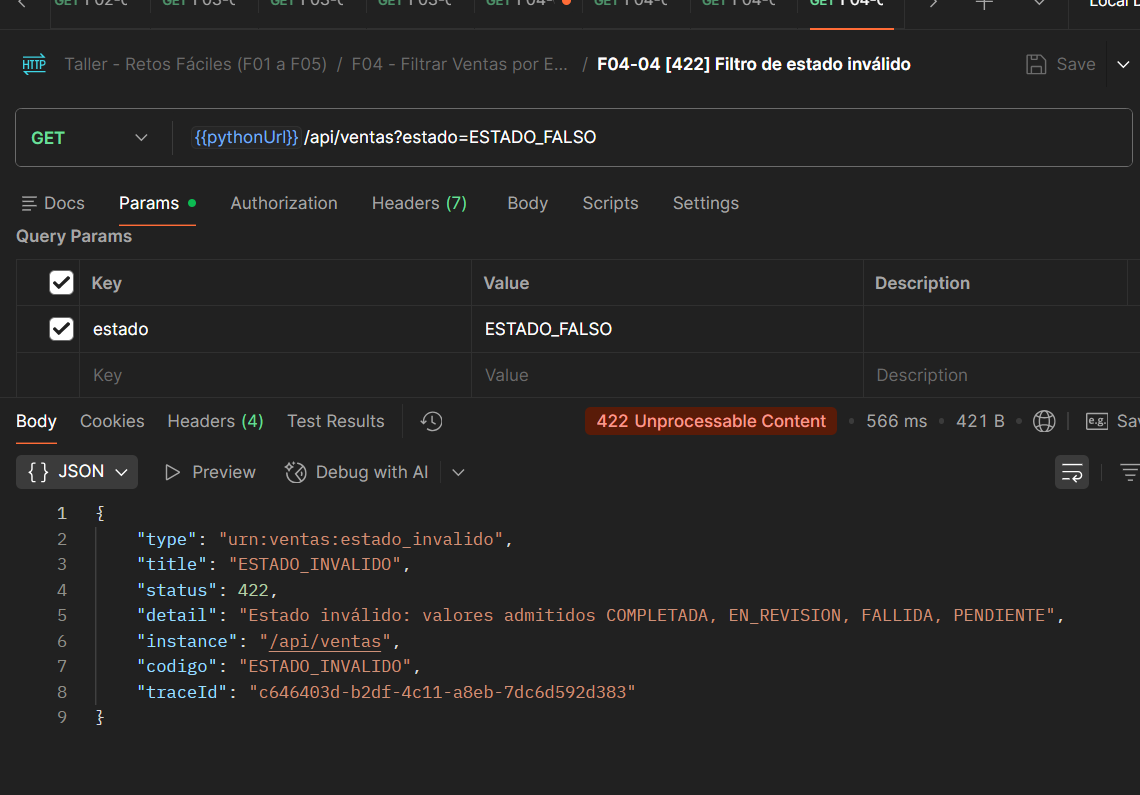
\includegraphics[width=0.95\textwidth]{imagenes/media/image12.png}
    \caption{F04-04: Rechazo por estado inválido ESTADO\_FALSO (422 Unprocessable Content).}
    \label{fig:f04_04}
\end{figure}

\subsubsection{5. Persistencia (MySQL)}
\begin{lstlisting}[language=SQL]
SELECT id, operacion_id, estado, precio_acordado FROM ventas WHERE usuario = 'admin-local' AND estado = 'COMPLETADA';
\end{lstlisting}

\begin{figure}[H]
    \centering
    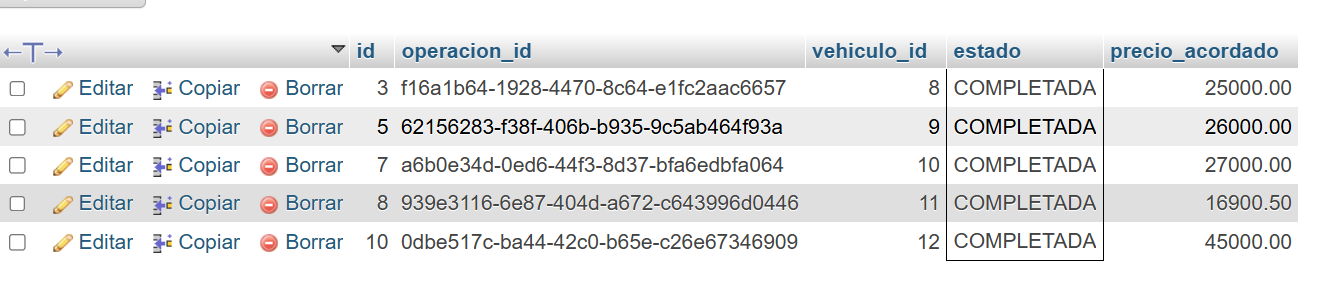
\includegraphics[width=0.95\textwidth]{imagenes/media/sql_f04.png}
    \caption{Evidencia SQL en MySQL: Registros de ventas filtrados estrictamente por estado COMPLETADA.}
    \label{fig:sql_f04}
\end{figure}

\subsubsection{6. Explicación}
La validación sintáctica y semántica del estado se realiza en la capa Router antes de ejecutar consultas. La normalización a mayúsculas evita discrepancias por formato y la cláusula SQL combinada garantiza que un usuario jamás vea estados ajenos.

\newpage
% ----------------------------------------------------------------------------
% F05
% ----------------------------------------------------------------------------
\subsection{F05 | Filtrar vehículos por marca y disponibilidad}
\textbf{Servicio y contrato:} Spring Boot $\cdot$ \texttt{GET /api/vehiculos?marca=...\&estado=DISPONIBLE}

\subsubsection{1. Diagnóstico}
En el servicio Java (\texttt{venta-vehiculos-api\_security}), el catálogo únicamente admitía filtrar por la marca del vehículo. Los clientes no podían consultar vehículos disponibles para reservar ni discriminar los ya vendidos o reservados.

\subsubsection{2. Diseño}
Se extendió el endpoint \texttt{GET /api/vehiculos} en Spring Boot para aceptar el parámetro opcional \texttt{estado}. Reglas:
\begin{itemize}
    \item Admitir los estados del dominio de negocio: \texttt{DISPONIBLE}, \texttt{RESERVADO} y \texttt{VENDIDO}.
    \item Soporte de 4 combinaciones: sin filtros, solo marca, solo estado, y ambos simultáneamente.
    \item Cualquier valor ajeno produce \texttt{400 Bad Request} con estructura de error RFC 7807 y código \texttt{ESTADO\_INVALIDO}.
\end{itemize}

\subsubsection{3. Implementación}
En \texttt{VehiculoController.java} y \texttt{VehiculoService.java}:
\begin{lstlisting}[language=Java]
@GetMapping
public ResponseEntity<?> listarVehiculos(
    @RequestParam(required = false) String marca,
    @RequestParam(required = false) String estado
) {
    if (estado != null) {
        String estNorm = estado.trim().toUpperCase();
        if (!ESTADOS_VALIDOS.contains(estNorm)) {
            return ResponseEntity.status(400)
                .contentType(MediaType.APPLICATION_PROBLEM_JSON)
                .body(Map.of("status", 400, "codigo", "ESTADO_INVALIDO", "detail", "Estado invalido"));
        }
    }
    return ResponseEntity.ok(vehiculoService.buscarVehiculos(marca, estado));
}
\end{lstlisting}

\subsubsection{4. Validación}
\begin{table}[H]
\centering
\small
\begin{tabularx}{\textwidth}{l p{4.5cm} p{2.5cm} c c X}
\toprule
\textbf{ID} & \textbf{Método / URL} & \textbf{Filtros} & \textbf{HTTP Esp.} & \textbf{HTTP Obt.} & \textbf{Resultado} \\
\midrule
F05-01 & \texttt{GET /api/vehiculos} & Ninguno & 200 & 200 & Catálogo completo de vehículos. \\
F05-02 & \texttt{GET /api/vehiculos?marca=Toyota} & Solo marca & 200 & 200 & Vehículos de marca Toyota. \\
F05-03 & \texttt{GET /api/vehiculos?estado=DISPONIBLE} & Solo estado & 200 & 200 & Vehículos en estado DISPONIBLE. \\
F05-04 & \texttt{GET /api/vehiculos?marca=Toyota\&estado=DISPONIBLE} & Marca y estado & 200 & 200 & Coincidencia exacta de ambos filtros. \\
F05-05 & \texttt{GET /api/vehiculos?estado=CHOCADO} & Estado no admitido & 400 & 400 & Rechazo controlado \texttt{ESTADO\_INVALIDO}. \\
\bottomrule
\end{tabularx}
\caption{Matriz de pruebas del reto F05.}
\end{table}

\begin{figure}[H]
    \centering
    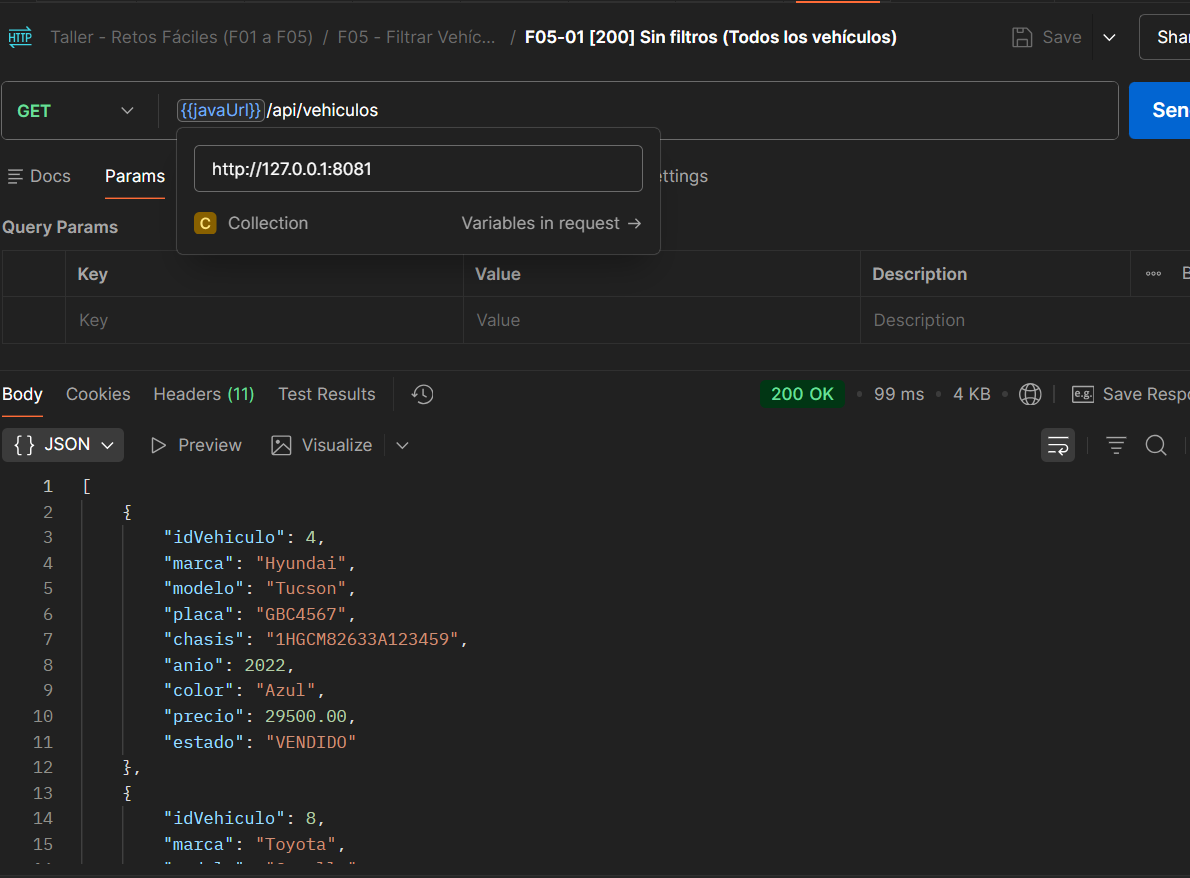
\includegraphics[width=0.95\textwidth]{imagenes/media/image13.png}
    \caption{F05-01: Catálogo sin filtros (200 OK).}
    \label{fig:f05_01}
\end{figure}

\begin{figure}[H]
    \centering
    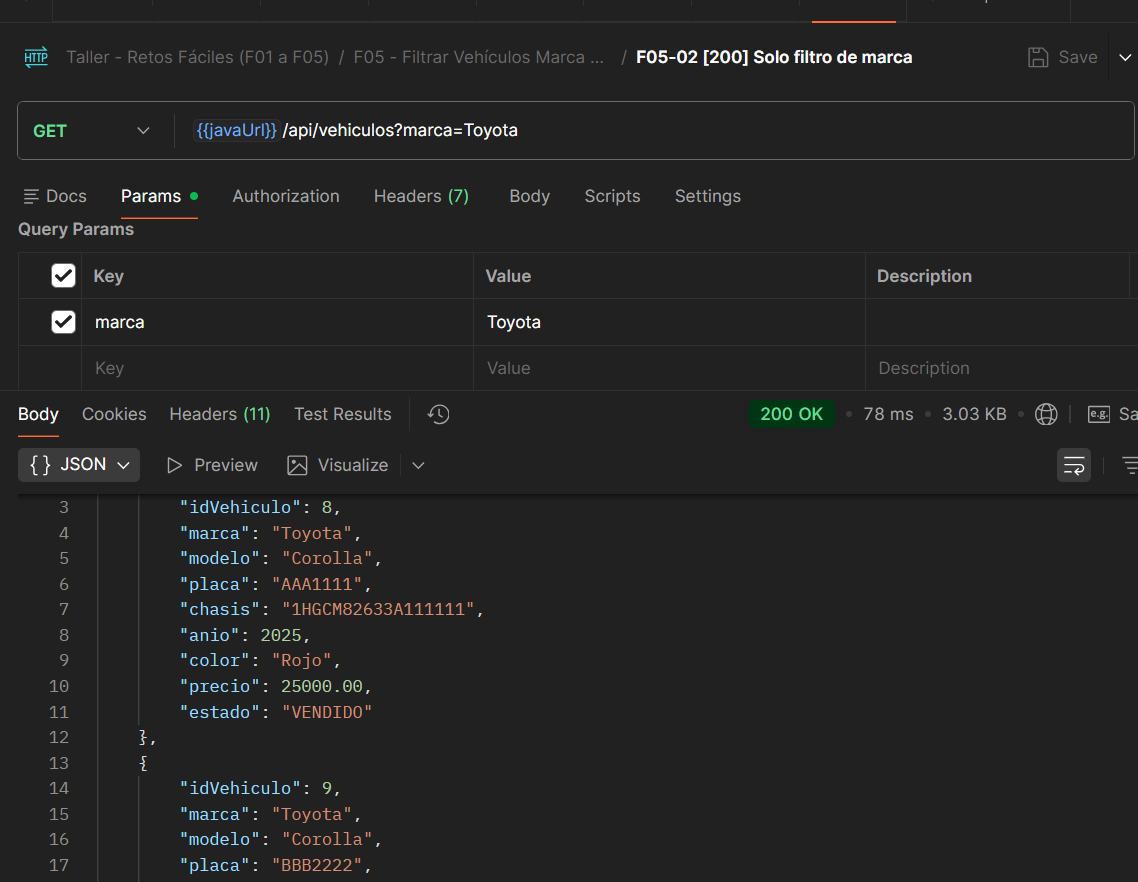
\includegraphics[width=0.95\textwidth]{imagenes/media/image14.png}
    \caption{F05-02: Filtrado únicamente por marca Toyota (200 OK).}
    \label{fig:f05_02}
\end{figure}

\begin{figure}[H]
    \centering
    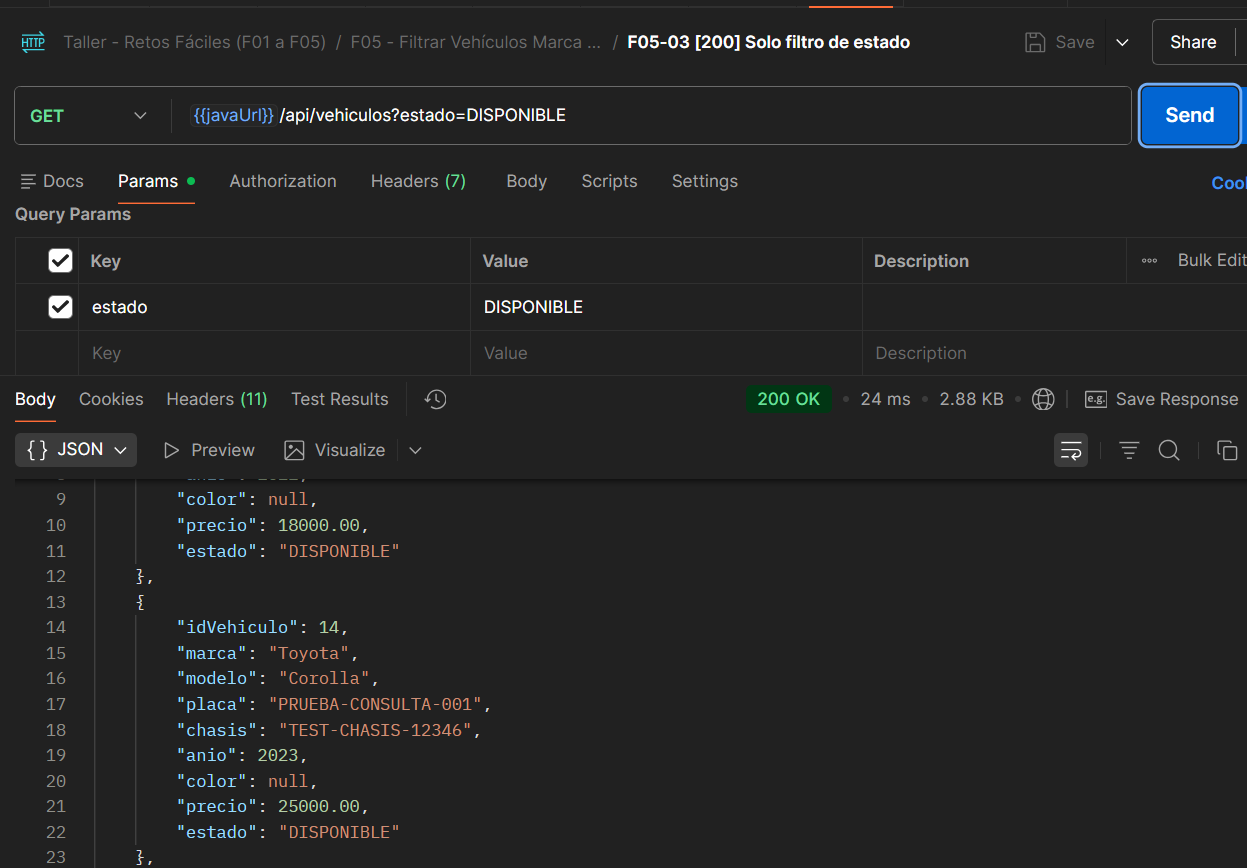
\includegraphics[width=0.95\textwidth]{imagenes/media/image15.png}
    \caption{F05-03: Filtrado únicamente por estado DISPONIBLE (200 OK).}
    \label{fig:f05_03}
\end{figure}

\begin{figure}[H]
    \centering
    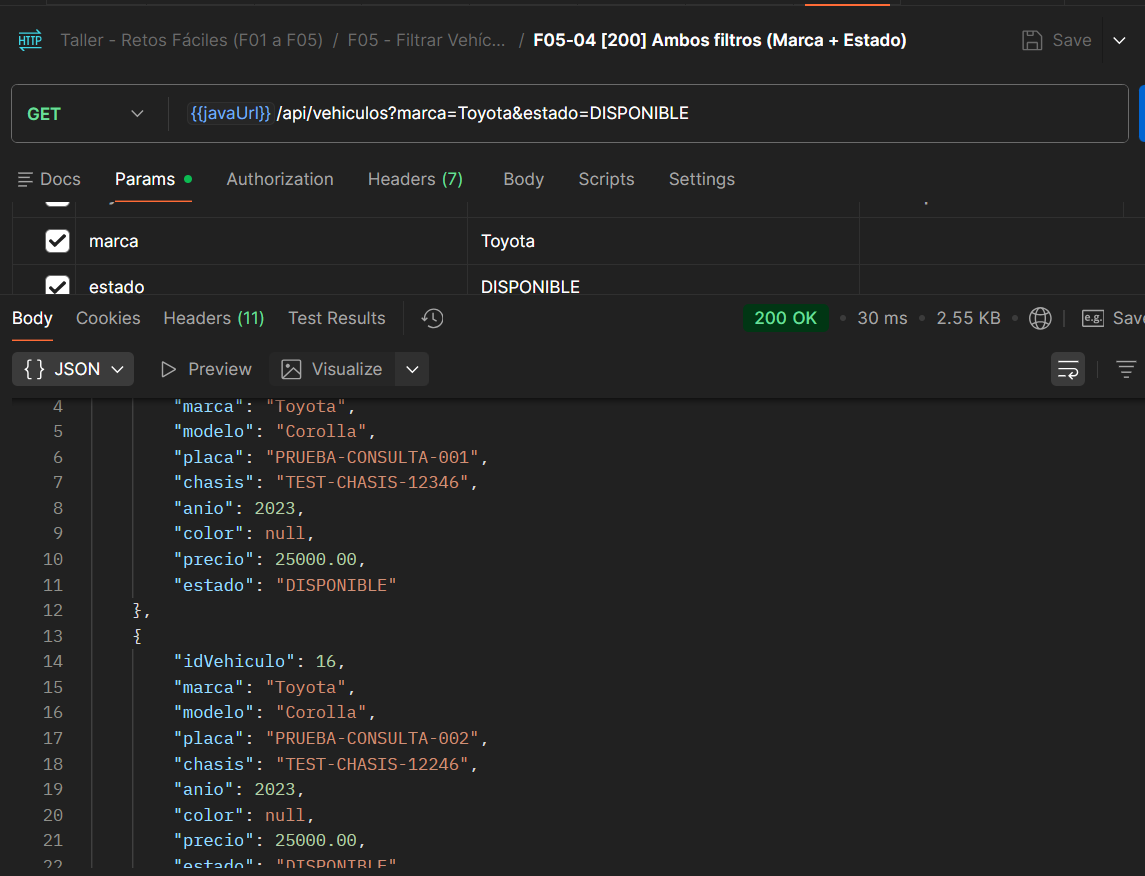
\includegraphics[width=0.95\textwidth]{imagenes/media/image16.png}
    \caption{F05-04: Filtrado combinado marca Toyota y estado DISPONIBLE (200 OK).}
    \label{fig:f05_04}
\end{figure}

\begin{figure}[H]
    \centering
    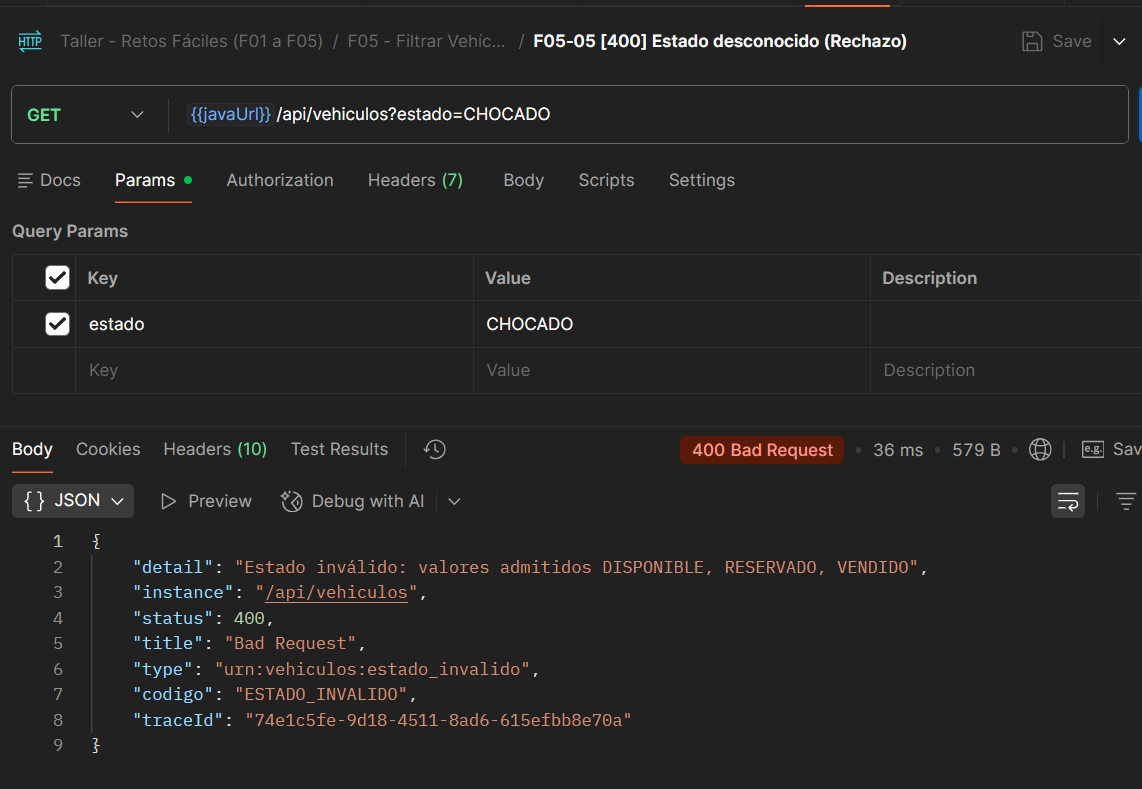
\includegraphics[width=0.95\textwidth]{imagenes/media/image17.png}
    \caption{F05-05: Rechazo por estado desconocido CHOCADO (400 Bad Request).}
    \label{fig:f05_05}
\end{figure}

\subsubsection{5. Persistencia (MySQL)}
\begin{lstlisting}[language=SQL]
SELECT id_vehiculo, marca, modelo, estado, precio FROM vehiculos WHERE marca = 'Toyota' AND estado = 'DISPONIBLE';
\end{lstlisting}

\begin{figure}[H]
    \centering
    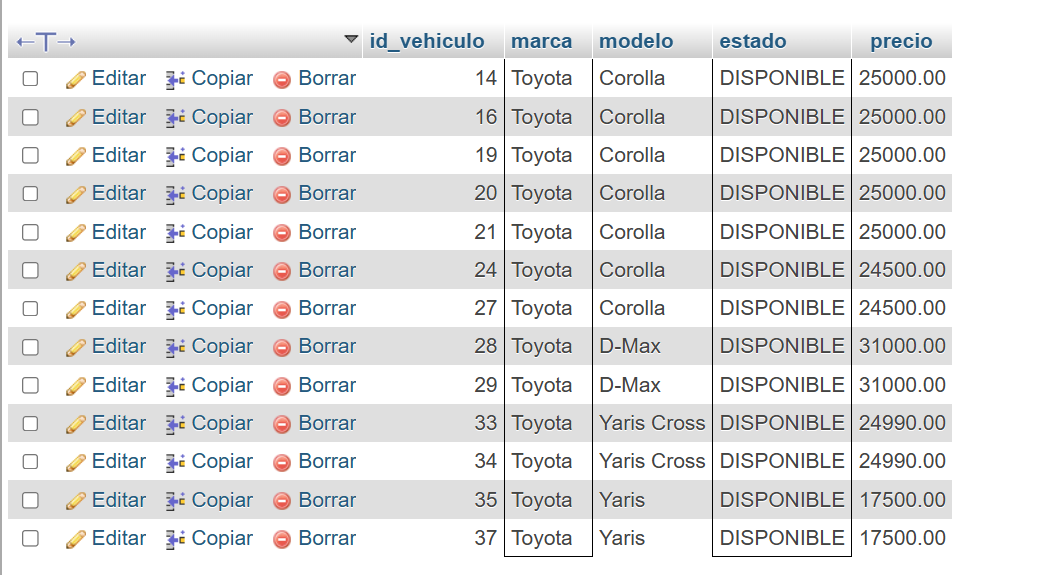
\includegraphics[width=0.95\textwidth]{imagenes/media/sql_f05.png}
    \caption{Evidencia SQL en MySQL: Vehículos de marca Toyota en estado DISPONIBLE en Spring Boot.}
    \label{fig:sql_f05}
\end{figure}

\subsubsection{6. Explicación}
La resolución se delegó al repositorio JPA mediante métodos derivados (\texttt{findByMarcaIgnoreCaseAndEstado}), permitiendo que Spring Data genere la consulta parametrizada con binding automático, evitando inyecciones SQL y optimizando la búsqueda por índices.

\newpage

% ============================================================================
% NIVEL 2 · RETOS DIFÍCILES (D06 - D10)
% ============================================================================
\section{Nivel 2 · Retos Difíciles (D06 a D10)}

% ----------------------------------------------------------------------------
% D06
% ----------------------------------------------------------------------------
\subsection{D06 | Paginación estable y segura de ventas}
\textbf{Servicio y contrato:} FastAPI $\cdot$ \texttt{GET /api/ventas?limit=10\&offset=0}

\subsubsection{1. Diagnóstico}
En escenarios de producción con cientos o miles de ventas, responder la totalidad de transacciones en una sola carga satura la memoria del servidor y el ancho de banda del cliente. Además, una paginación que carezca de límites máximos permite a usuarios malintencionados solicitar miles de filas en una sola petición (denegación de servicio por consumo de recursos).

\subsubsection{2. Diseño}
Se diseñó una estrategia de paginación basada en parámetros \texttt{limit} y \texttt{offset}:
\begin{itemize}
    \item Rango permitido: \texttt{limit} entre 1 y 50 inclusive. Cualquier valor menor a 1 o mayor a 50 retorna \texttt{422 LIMITE\_INVALIDO}.
    \item Restricción: \texttt{offset} no puede ser negativo ($\ge 0$); en caso contrario retorna \texttt{422 OFFSET\_INVALIDO}.
    \item Formato estructurado: Retorna \texttt{\{"items": [...], "total": N, "limit": L, "offset": O\}}.
    \item Compatibilidad: Si no se envían \texttt{limit} ni \texttt{offset}, se preserva el listado plano original de los retos F03/F04.
\end{itemize}

\subsubsection{3. Implementación}
\begin{lstlisting}[language=Python]
if limit is not None or offset is not None:
    l = limit if limit is not None else 10
    o = offset if offset is not None else 0
    if l < 1 or l > 50:
        raise ApiError(422, "LIMITE_INVALIDO", "Limit debe estar entre 1 y 50")
    if o < 0:
        raise ApiError(422, "OFFSET_INVALIDO", "Offset no puede ser negativo")
    total = repo.contar_propias(u["usuario"], estado=estado)
    ventas = repo.listar_propias(u["usuario"], estado=estado, limit=l, offset=o)
    return {"items": [service.salida(v) for v in ventas], "total": total, "limit": l, "offset": o}
\end{lstlisting}

\subsubsection{4. Validación}
\begin{table}[H]
\centering
\small
\begin{tabularx}{\textwidth}{l p{4cm} p{2.5cm} c c X}
\toprule
\textbf{ID} & \textbf{Método / URL} & \textbf{Parámetros} & \textbf{HTTP Esp.} & \textbf{HTTP Obt.} & \textbf{Resultado} \\
\midrule
D06-01 & \texttt{GET /api/ventas} & \texttt{limit=2\&offset=0} & 200 & 200 & Página 1 con los 2 registros más recientes. \\
D06-02 & \texttt{GET /api/ventas} & \texttt{limit=2\&offset=2} & 200 & 200 & Página 2 con los siguientes 2 registros sin duplicados. \\
D06-03 & \texttt{GET /api/ventas} & \texttt{limit=100} & 422 & 422 & Rechazo por límite excesivo ($>50$). \\
D06-04 & \texttt{GET /api/ventas} & \texttt{offset=-1} & 422 & 422 & Rechazo por desplazamiento negativo. \\
\bottomrule
\end{tabularx}
\caption{Matriz de pruebas del reto D06.}
\end{table}

\begin{figure}[H]
    \centering
    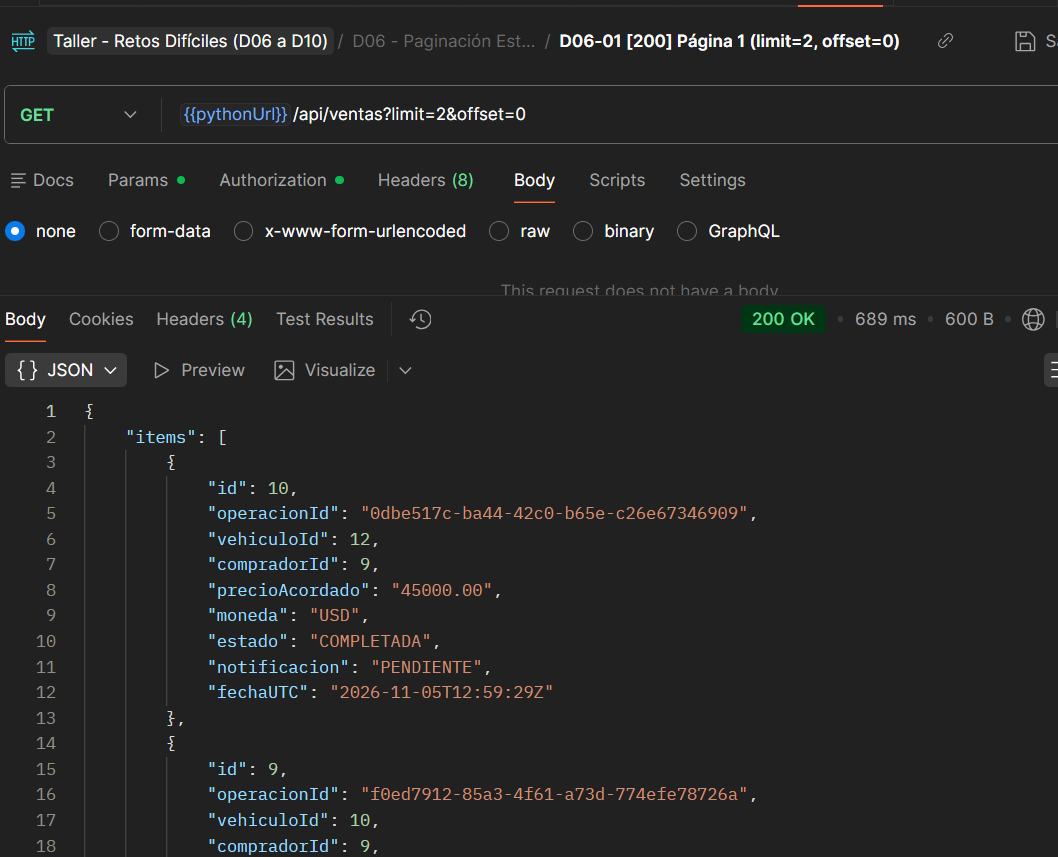
\includegraphics[width=0.95\textwidth]{imagenes/media/image18.png}
    \caption{D06-01: Página 1 con limit=2 y offset=0 (200 OK).}
    \label{fig:d06_01}
\end{figure}

\begin{figure}[H]
    \centering
    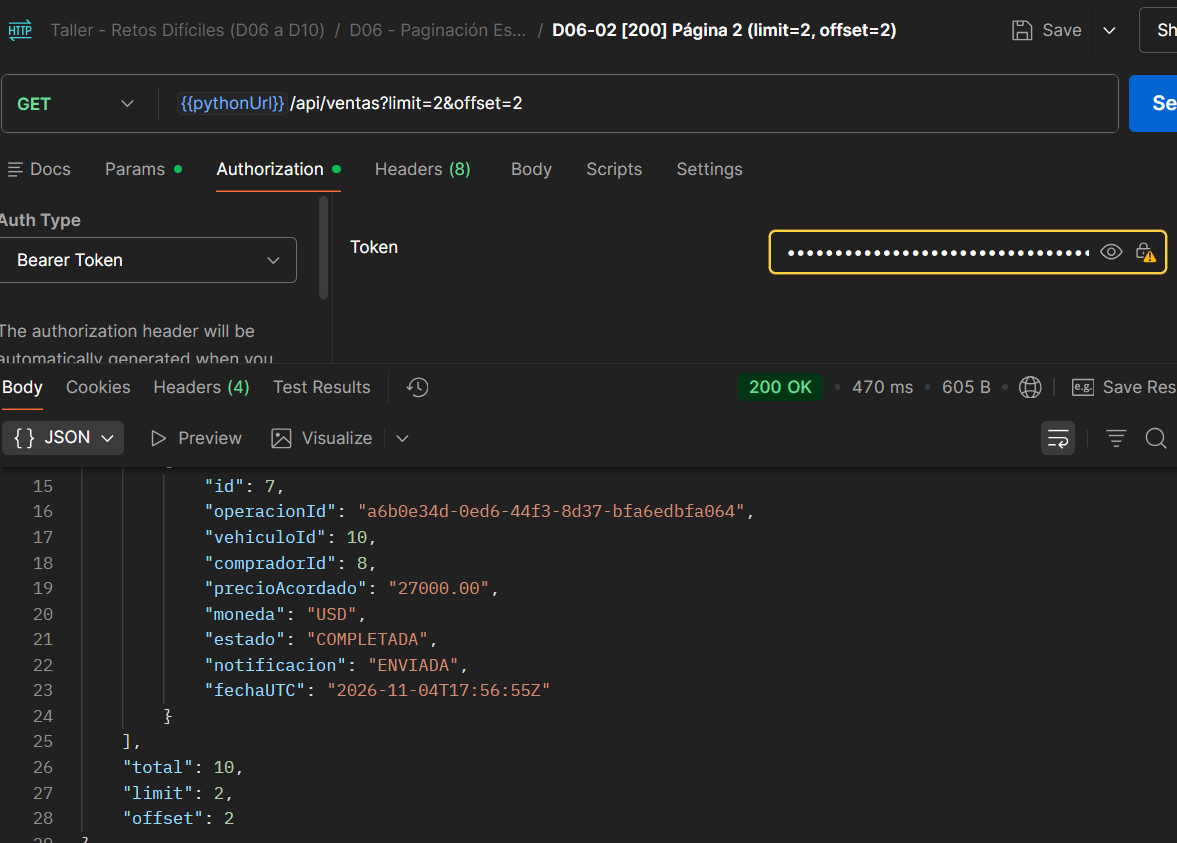
\includegraphics[width=0.95\textwidth]{imagenes/media/image19.png}
    \caption{D06-02: Página 2 con limit=2 y offset=2 (200 OK).}
    \label{fig:d06_02}
\end{figure}

\begin{figure}[H]
    \centering
    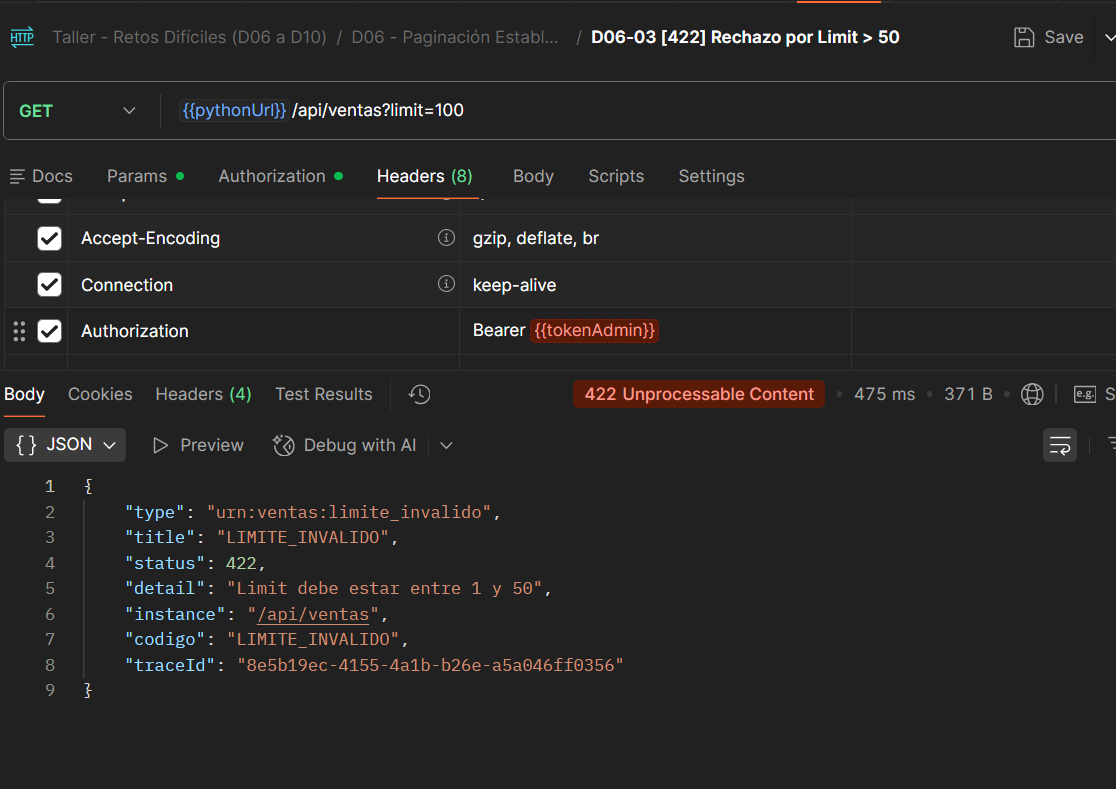
\includegraphics[width=0.95\textwidth]{imagenes/media/image20.png}
    \caption{D06-03: Rechazo por limit mayor a 50 (422 Unprocessable Content).}
    \label{fig:d06_03}
\end{figure}

\begin{figure}[H]
    \centering
    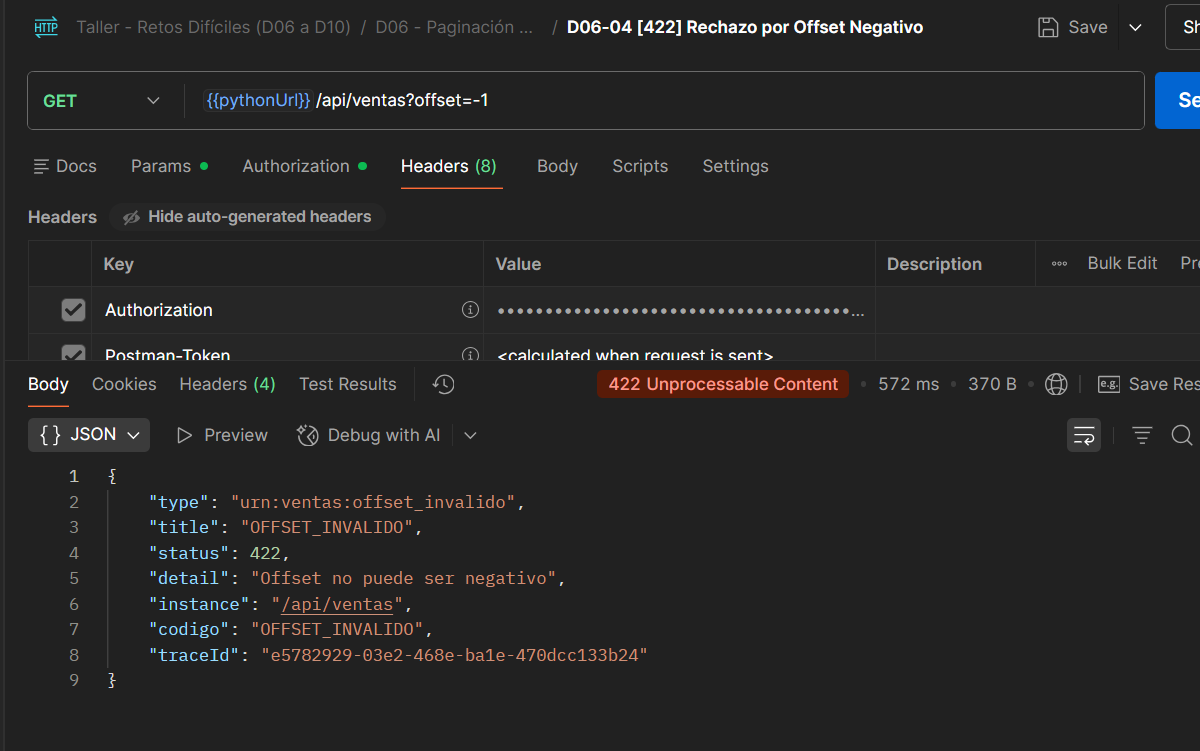
\includegraphics[width=0.95\textwidth]{imagenes/media/image21.png}
    \caption{D06-04: Rechazo por offset negativo (422 Unprocessable Content).}
    \label{fig:d06_04}
\end{figure}

\subsubsection{5. Persistencia (MySQL)}
\begin{lstlisting}[language=SQL]
SELECT COUNT(*) FROM ventas WHERE usuario = 'admin-local';
SELECT * FROM ventas WHERE usuario = 'admin-local' ORDER BY fecha DESC, id DESC LIMIT 2 OFFSET 0;
\end{lstlisting}

\begin{figure}[H]
    \centering
    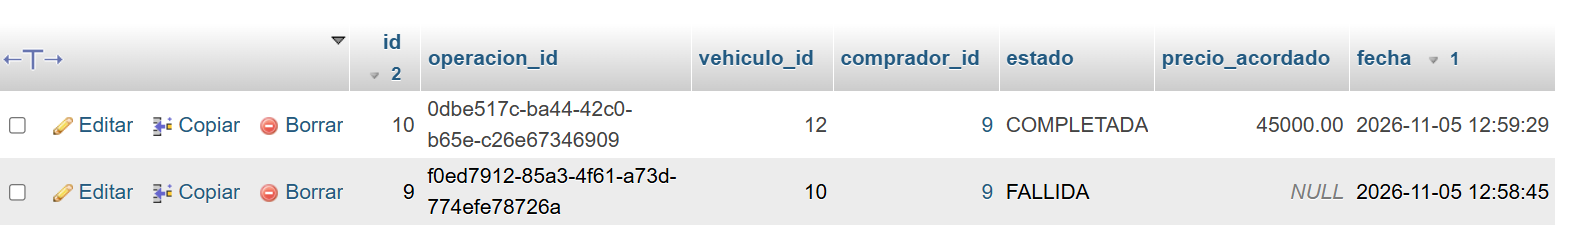
\includegraphics[width=0.95\textwidth]{imagenes/media/sql_d06_detalle.png}
    \caption{Evidencia SQL en MySQL: Detalle de las ventas paginadas correspondientes a la Página 1.}
    \label{fig:sql_d06}
\end{figure}

\subsubsection{6. Explicación}
La combinación de \texttt{COUNT} y paginación en el motor relacional proporciona el total global de coincidencias para que la interfaz construya su paginador numérico. El ordenamiento estricto evita el solapamiento o pérdida de registros entre páginas consecutivas.

\newpage
% ----------------------------------------------------------------------------
% D07
% ----------------------------------------------------------------------------
\subsection{D07 | Buscar compradores por nombre o documento}
\textbf{Servicio y contrato:} FastAPI $\cdot$ \texttt{GET /api/compradores?buscar=texto}

\subsubsection{1. Diagnóstico}
El listado de compradores de F01 recuperaba todos los clientes del usuario sin capacidad de filtrar, dificultando la localización de personas en libretas grandes por su cédula o nombre.

\subsubsection{2. Diseño}
Se integró el parámetro de búsqueda parcial \texttt{buscar}. Reglas clave:
\begin{itemize}
    \item Búsqueda no sensible a mayúsculas (\texttt{ILIKE} / \texttt{LIKE}) sobre \texttt{nombre} o \texttt{documento}.
    \item Aislamiento estricto: La condición \texttt{usuario = :u} debe envolver la cláusula con un operador \texttt{AND (nombre LIKE :b OR documento LIKE :b)}.
    \item Resistencia a inyección SQL: El término se pasa obligatoriamente como parámetro compilado por SQLAlchemy, jamás mediante concatenación directa de cadenas.
\end{itemize}

\subsubsection{3. Implementación}
En \texttt{CompradorRepository.listar\_por\_usuario}:
\begin{lstlisting}[language=Python]
def listar_por_usuario(self, usuario: str, buscar: str | None = None):
    stmt = select(Comprador).where(Comprador.usuario == usuario)
    if buscar and buscar.strip():
        term = f"%{buscar.strip()}%"
        stmt = stmt.where(or_(Comprador.nombre.ilike(term), Comprador.documento.ilike(term)))
    stmt = stmt.order_by(Comprador.id.asc())
    return self.db.scalars(stmt).all()
\end{lstlisting}

\subsubsection{4. Validación}
\begin{table}[H]
\centering
\small
\begin{tabularx}{\textwidth}{l p{4cm} p{3cm} c c X}
\toprule
\textbf{ID} & \textbf{Método / URL} & \textbf{Criterio Búsqueda} & \textbf{HTTP Esp.} & \textbf{HTTP Obt.} & \textbf{Resultado} \\
\midrule
D07-01 & \texttt{GET /api/compradores} & \texttt{buscar=Test} & 200 & 200 & Coincidencia por nombre. \\
D07-02 & \texttt{GET /api/compradores} & \texttt{buscar=1234} & 200 & 200 & Coincidencia por documento. \\
D07-03 & \texttt{GET /api/compradores} & \texttt{buscar=INEXISTENTE} & 200 & 200 & Lista vacía \texttt{[]}. \\
D07-04 & \texttt{GET /api/compradores} & \texttt{buscar=' OR '1'='1} & 200 & 200 & Lista vacía \texttt{[]} (inyección neutralizada). \\
\bottomrule
\end{tabularx}
\caption{Matriz de pruebas del reto D07.}
\end{table}

\begin{figure}[H]
    \centering
    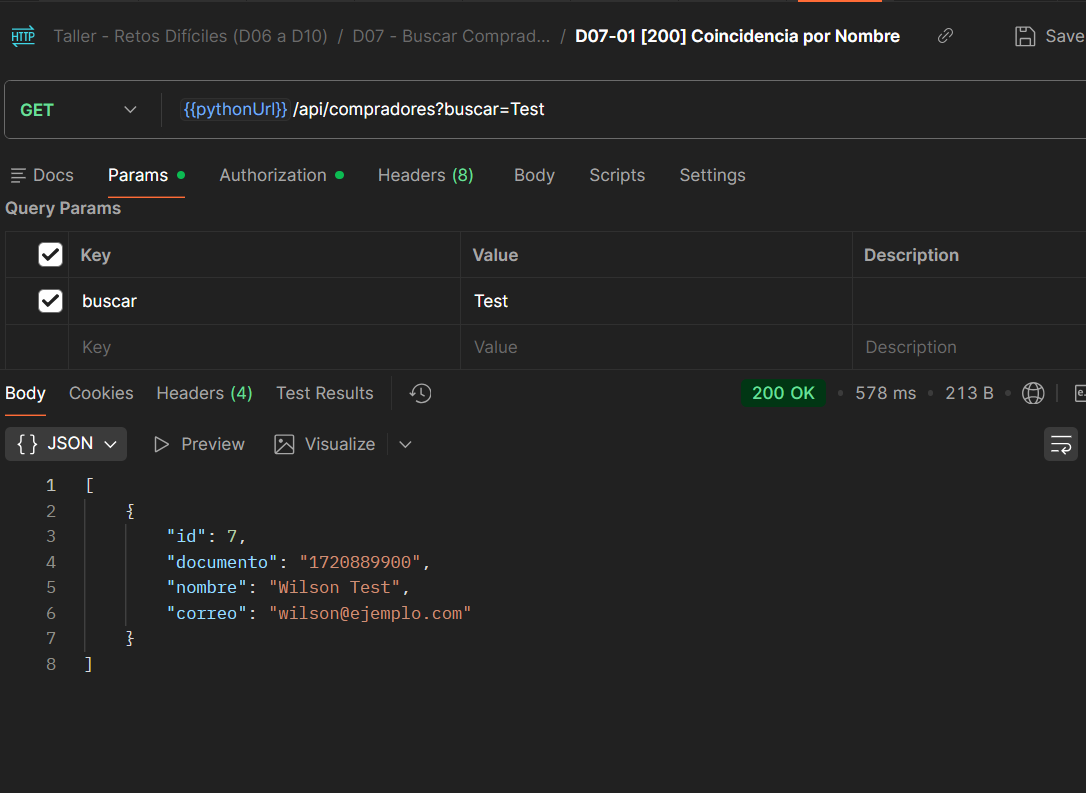
\includegraphics[width=0.95\textwidth]{imagenes/media/image22.png}
    \caption{D07-01: Coincidencia por nombre 'Test' (200 OK).}
    \label{fig:d07_01}
\end{figure}

\begin{figure}[H]
    \centering
    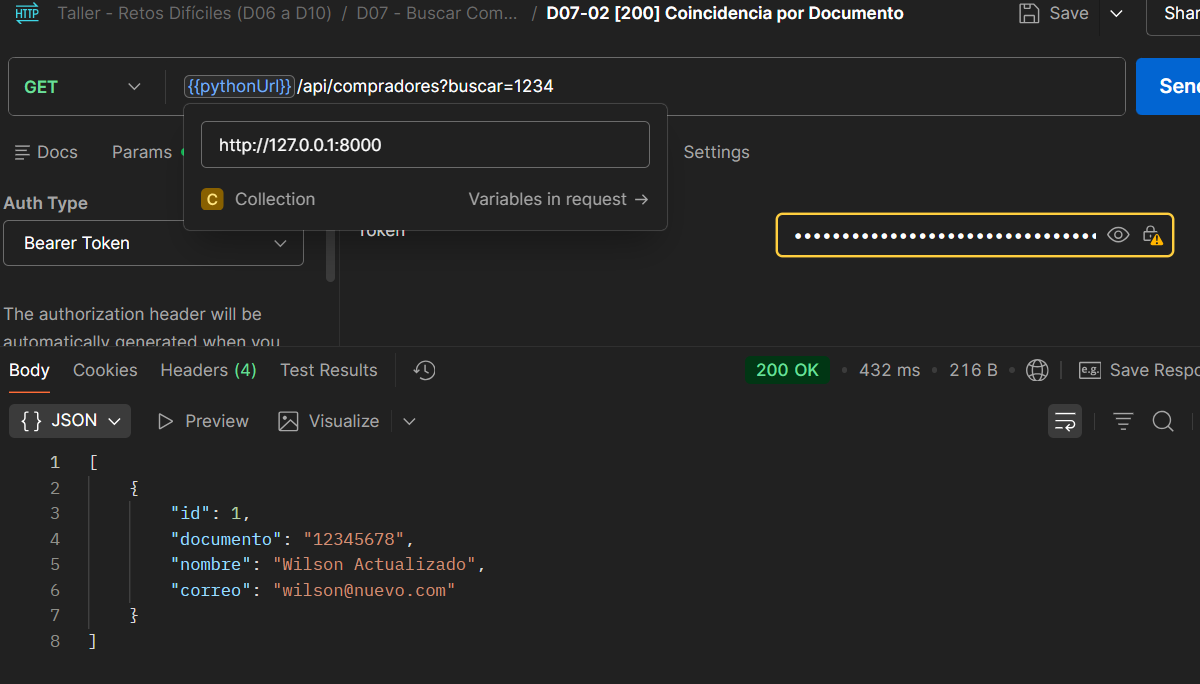
\includegraphics[width=0.95\textwidth]{imagenes/media/image23.png}
    \caption{D07-02: Coincidencia por documento '1234' (200 OK).}
    \label{fig:d07_02}
\end{figure}

\begin{figure}[H]
    \centering
    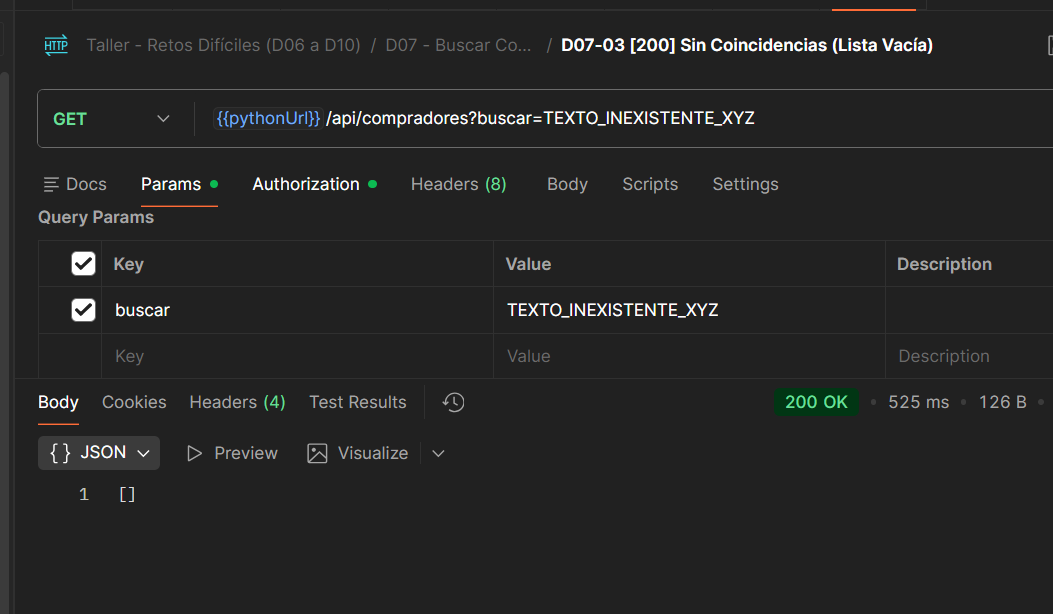
\includegraphics[width=0.95\textwidth]{imagenes/media/image24.png}
    \caption{D07-03: Búsqueda sin coincidencias devolviendo lista vacía (200 OK []).}
    \label{fig:d07_03}
\end{figure}

\begin{figure}[H]
    \centering
    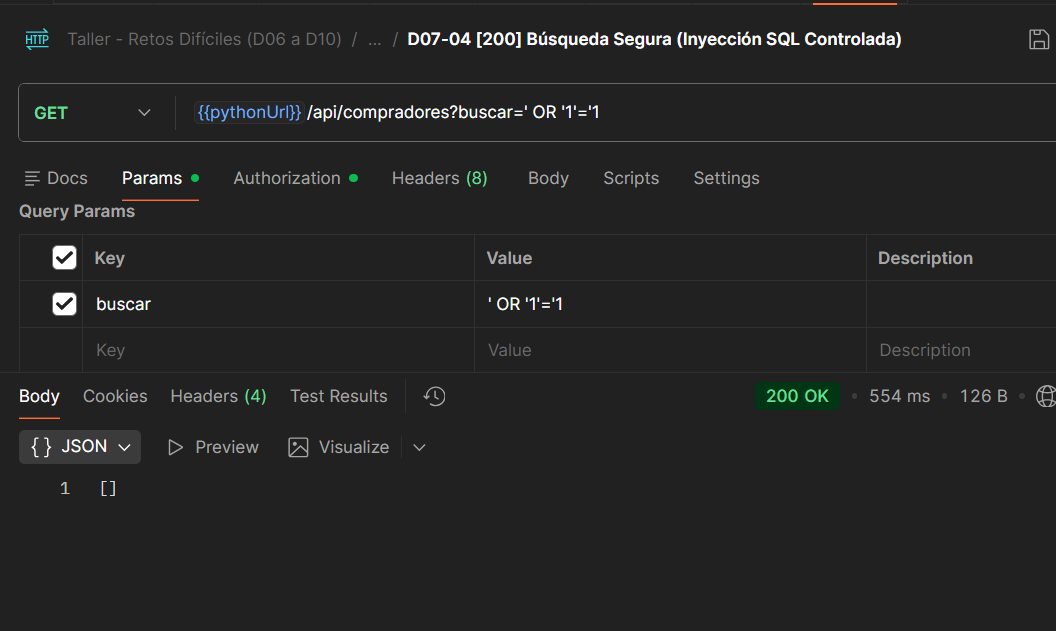
\includegraphics[width=0.95\textwidth]{imagenes/media/image25.png}
    \caption{D07-04: Inyección SQL neutralizada devolviendo lista vacía (200 OK []).}
    \label{fig:d07_04}
\end{figure}

\subsubsection{5. Persistencia (MySQL)}
\begin{lstlisting}[language=SQL]
SELECT * FROM compradores WHERE usuario = 'admin-local' AND (nombre LIKE '%Test%' OR documento LIKE '%Test%');
\end{lstlisting}

\begin{figure}[H]
    \centering
    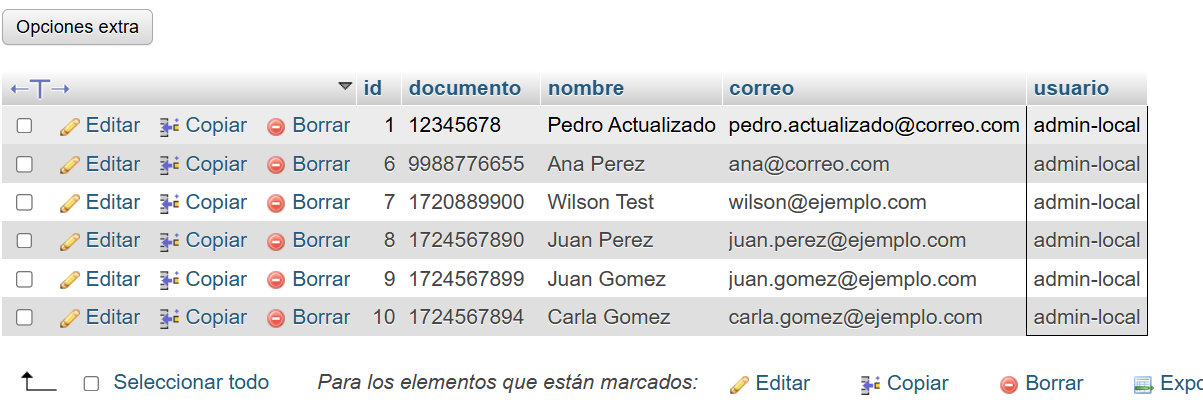
\includegraphics[width=0.95\textwidth]{imagenes/media/sql_f01_d07.png}
    \caption{Evidencia SQL en MySQL: Compradores recuperables mediante coincidencia por nombre o documento.}
    \label{fig:sql_d07}
\end{figure}

\subsubsection{6. Explicación}
La prueba D07-04 demuestra de manera fehaciente la seguridad de la solución: al inyectar \texttt{' OR '1'='1}, SQLAlchemy trata los caracteres literalmente como parte del valor a buscar y no altera la gramática SQL, devolviendo cero coincidencias sin exponer información ajena.

\newpage
% ----------------------------------------------------------------------------
% D08
% ----------------------------------------------------------------------------
\subsection{D08 | Actualizar comprador sin cambiar documento}
\textbf{Servicio y contrato:} FastAPI $\cdot$ \texttt{PUT /api/compradores/\{id\}}

\subsubsection{1. Diagnóstico}
No existía ningún mecanismo para actualizar la información de contacto de un comprador. Permitir una actualización descontrolada podría corromper el número de cédula o documento de identidad, violando la integridad de facturación y las ventas previamente asociadas.

\subsubsection{2. Diseño}
Se diseñó el endpoint \texttt{PUT /api/compradores/\{id\}} con un esquema DTO específico \texttt{ActualizarComprador}:
\begin{itemize}
    \item Inmutabilidad: El campo \texttt{documento} no existe en el esquema de entrada; el servicio únicamente modifica \texttt{nombre} y \texttt{correo}.
    \item Validación estricta: Formato de correo validado con expresión regular RFC. Si el correo es inválido, retorna \texttt{422 VALIDACION}.
    \item Propiedad: El comprador debe existir (\texttt{404}) y pertenecer al usuario o el usuario tener rol administrador (\texttt{403}).
\end{itemize}

\subsubsection{3. Implementación}
En \texttt{app/schemas.py} y \texttt{app/routers/ventas.py}:
\begin{lstlisting}[language=Python]
class ActualizarComprador(BaseModel):
    nombre: Annotated[str, Field(min_length=2, max_length=150)]
    correo: Annotated[str, Field(pattern=r"^[^@\s]+@[^@\s]+\.[^@\s]+$")]

@router.put("/compradores/{id}")
def actualizar_comprador(id: int, d: ActualizarComprador, u=Depends(identidad)):
    vendedor(u)
    with SessionLocal.begin() as db:
        c = CompradorRepository(db).por_id(id)
        if c is None:
            raise ApiError(404, "COMPRADOR_NO_EXISTE", "Comprador inexistente")
        propietario(u, c.usuario)
        c.nombre = d.nombre
        c.correo = d.correo
        return {"id": c.id, "documento": c.documento, "nombre": c.nombre, "correo": c.correo}
\end{lstlisting}

\subsubsection{4. Validación}
\begin{table}[H]
\centering
\small
\begin{tabularx}{\textwidth}{l p{3.5cm} p{3cm} c c X}
\toprule
\textbf{ID} & \textbf{Método / URL} & \textbf{Cuerpo / Caso} & \textbf{HTTP Esp.} & \textbf{HTTP Obt.} & \textbf{Resultado} \\
\midrule
D08-01 & \texttt{PUT /api/compradores/1} & Nombre y correo válidos & 200 & 200 & Comprador actualizado, documento intacto. \\
D08-02 & \texttt{PUT /api/compradores/1} & Correo sin arroba & 422 & 422 & Rechazo \texttt{VALIDACION}. \\
D08-03 & \texttt{PUT /api/compradores/99999} & ID inexistente & 404 & 404 & Rechazo \texttt{COMPRADOR\_NO\_EXISTE}. \\
\bottomrule
\end{tabularx}
\caption{Matriz de pruebas del reto D08.}
\end{table}

\begin{figure}[H]
    \centering
    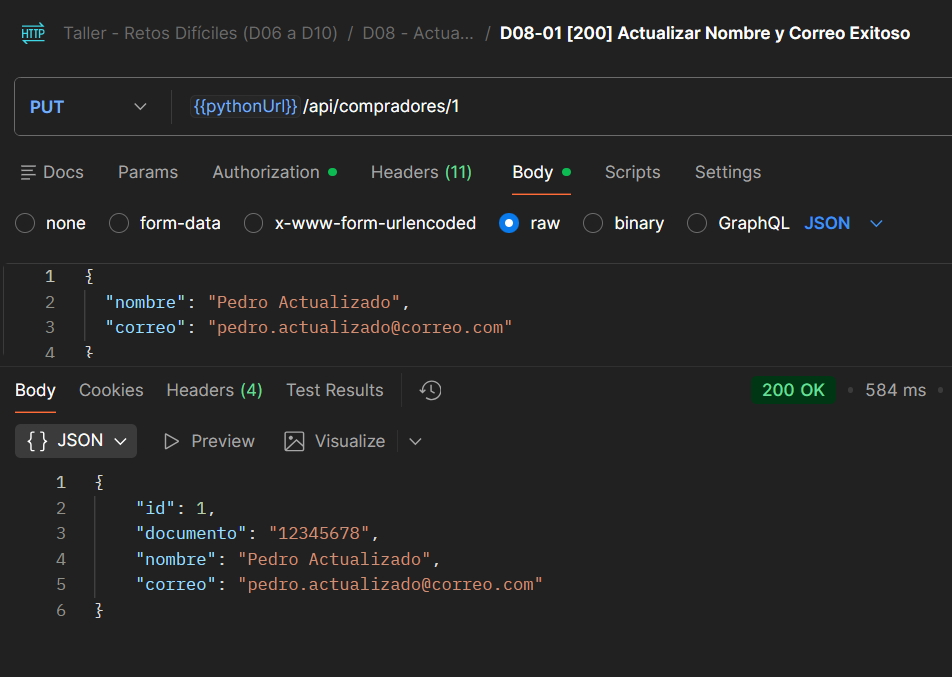
\includegraphics[width=0.95\textwidth]{imagenes/media/image26.png}
    \caption{D08-01: Actualización exitosa de nombre y correo (200 OK).}
    \label{fig:d08_01}
\end{figure}

\begin{figure}[H]
    \centering
    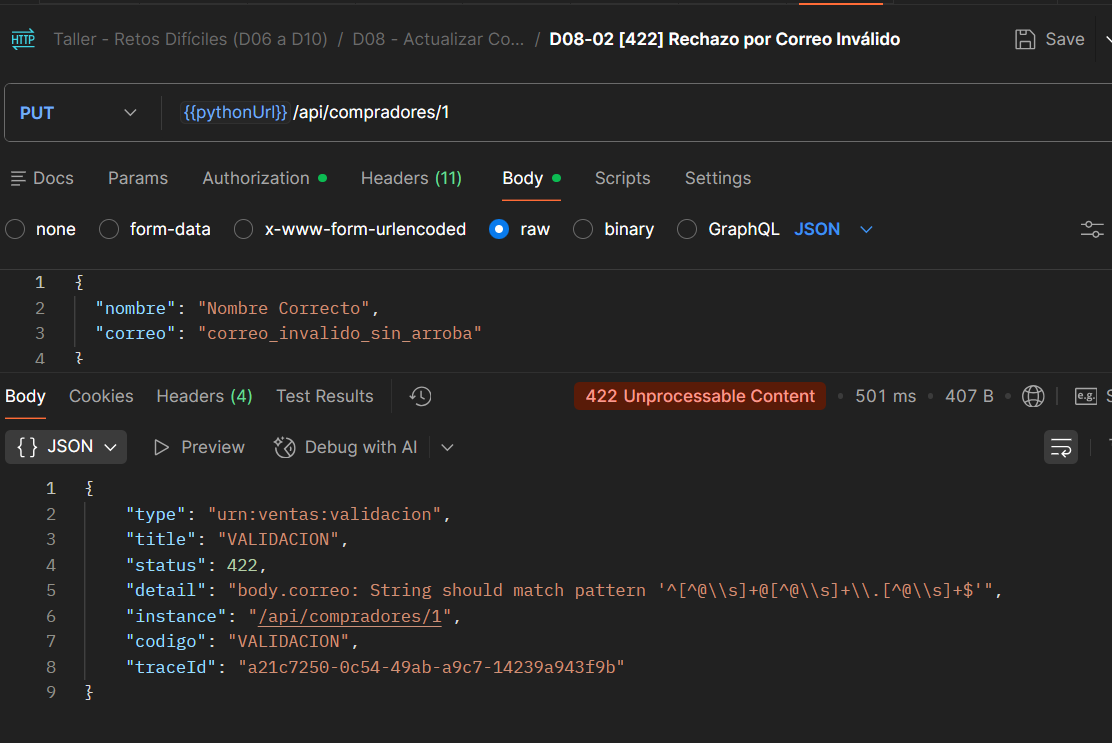
\includegraphics[width=0.95\textwidth]{imagenes/media/image27.png}
    \caption{D08-02: Rechazo por correo inválido sin arroba (422 Unprocessable Content).}
    \label{fig:d08_02}
\end{figure}

\begin{figure}[H]
    \centering
    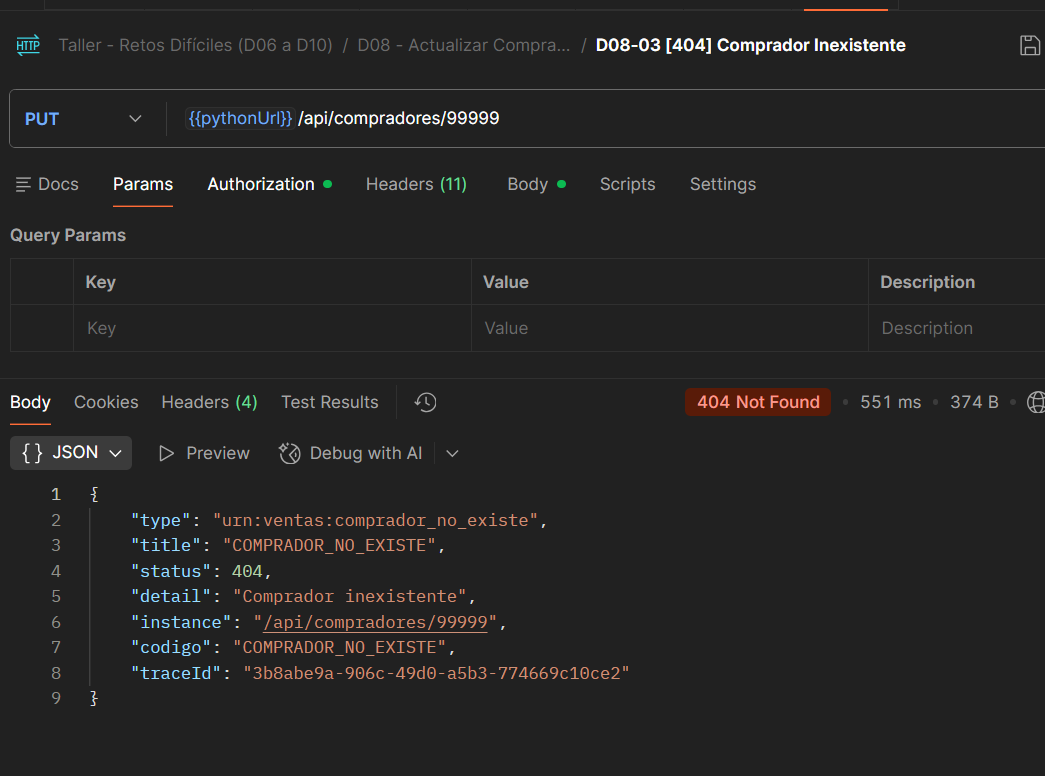
\includegraphics[width=0.95\textwidth]{imagenes/media/image28.png}
    \caption{D08-03: Rechazo por comprador inexistente (404 Not Found).}
    \label{fig:d08_03}
\end{figure}

\subsubsection{5. Persistencia (MySQL)}
\begin{lstlisting}[language=SQL]
SELECT id, documento, nombre, correo, usuario FROM compradores WHERE id = 1;
\end{lstlisting}

\begin{figure}[H]
    \centering
    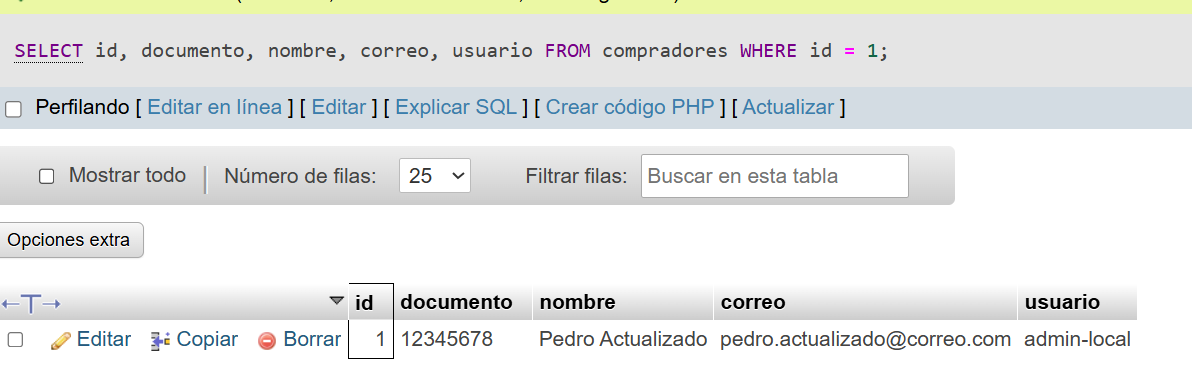
\includegraphics[width=0.95\textwidth]{imagenes/media/sql_f02_d08.png}
    \caption{Evidencia SQL en MySQL: Persistencia tras PUT. Documento 12345678 inmutable, nombre y correo actualizados.}
    \label{fig:sql_d08}
\end{figure}
El resultado en MySQL demuestra que \texttt{nombre} cambió a \texttt{"Pedro Actualizado"} y \texttt{correo} a \texttt{"pedro.actualizado@correo.com"}, mientras que el documento \texttt{"12345678"} permaneció intacto.

\subsubsection{6. Explicación}
La arquitectura por capas separa el modelo de datos relacional del DTO de entrada. Al excluir intencionalmente el atributo \texttt{documento} del DTO, no existe ninguna ruta de ejecución que permita modificarlo mediante esta operación.

\newpage
% ----------------------------------------------------------------------------
% D09
% ----------------------------------------------------------------------------
\subsection{D09 | Resumen numérico de ventas del usuario}
\textbf{Servicio y contrato:} FastAPI $\cdot$ \texttt{GET /api/ventas/resumen}

\subsubsection{1. Diagnóstico}
Los vendedores necesitaban conocer rápidamente sus métricas operativas (ventas completadas, ingresos totales generados, ventas fallidas y pendientes). Sin este servicio, el frontend debía solicitar todo el historial y recalcular las sumas localmente, exponiéndose a errores de redondeo de punto flotante.

\subsubsection{2. Diseño}
Se diseñó la ruta estática \texttt{GET /api/ventas/resumen}. Puntos críticos de diseño:
\begin{itemize}
    \item Prevención de colisión de rutas: En FastAPI, las rutas específicas (\texttt{/ventas/resumen}) deben registrarse obligatoriamente antes de las rutas parametrizadas (\texttt{/ventas/\{id\}}); de lo contrario, el framework intentaría castear la palabra \texttt{'resumen'} como un entero \texttt{id}.
    \item Precisión financiera: Uso obligatorio de \texttt{Decimal} para la acumulación monetaria.
    \item Regla contable: Las ventas en estado \texttt{FALLIDA} o \texttt{PENDIENTE} se excluyen estrictamente de la suma de \texttt{totalIngresos}.
\end{itemize}

\subsubsection{3. Implementación}
\begin{lstlisting}[language=Python]
@router.get("/ventas/resumen")
def resumen_ventas(u=Depends(identidad)):
    vendedor(u)
    with SessionLocal() as db:
        ventas = VentaRepository(db).listar_propias(u["usuario"])
        completadas = 0
        total_ingresos = Decimal("0.00")
        pendientes = sum(1 for v in ventas if v.estado == "PENDIENTE")
        en_revision = sum(1 for v in ventas if v.estado == "EN_REVISION")
        fallidas = sum(1 for v in ventas if v.estado == "FALLIDA")
        for v in ventas:
            if v.estado == "COMPLETADA":
                completadas += 1
                if v.precio_acordado is not None:
                    total_ingresos += v.precio_acordado
        return {
            "usuario": u["usuario"], "completadas": completadas,
            "totalIngresos": str(total_ingresos), "pendientes": pendientes,
            "enRevision": en_revision, "fallidas": fallidas, "totalVentas": len(ventas)
        }
\end{lstlisting}

\subsubsection{4. Validación}
\begin{table}[H]
\centering
\small
\begin{tabularx}{\textwidth}{l p{4cm} p{2.5cm} c c X}
\toprule
\textbf{ID} & \textbf{Método / URL} & \textbf{Auth} & \textbf{HTTP Esp.} & \textbf{HTTP Obt.} & \textbf{Resultado} \\
\midrule
D09-01 & \texttt{GET /api/ventas/resumen} & Token válido & 200 & 200 & Métricas numéricas consistentes con MySQL. \\
D09-02 & \texttt{GET /api/ventas/resumen} & Sin Token & 401 & 401 & Rechazo \texttt{NO\_AUTENTICADO}. \\
\bottomrule
\end{tabularx}
\caption{Matriz de pruebas del reto D09.}
\end{table}

\begin{figure}[H]
    \centering
    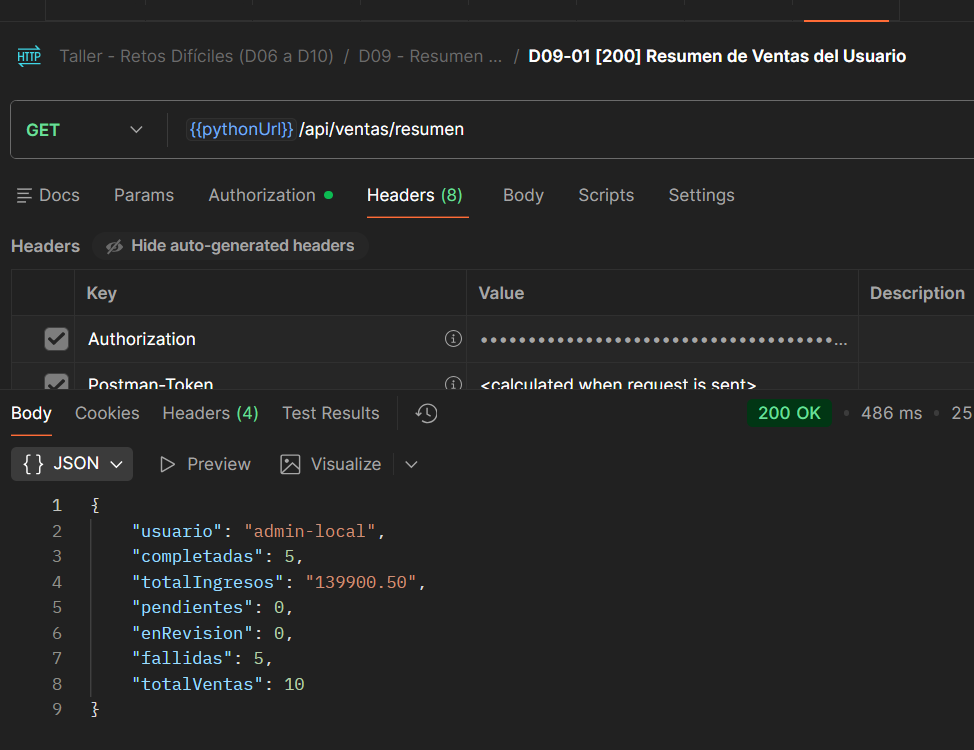
\includegraphics[width=0.95\textwidth]{imagenes/media/image29.png}
    \caption{D09-01: Resumen numérico y financiero de ventas del usuario (200 OK).}
    \label{fig:d09_01}
\end{figure}

\begin{figure}[H]
    \centering
    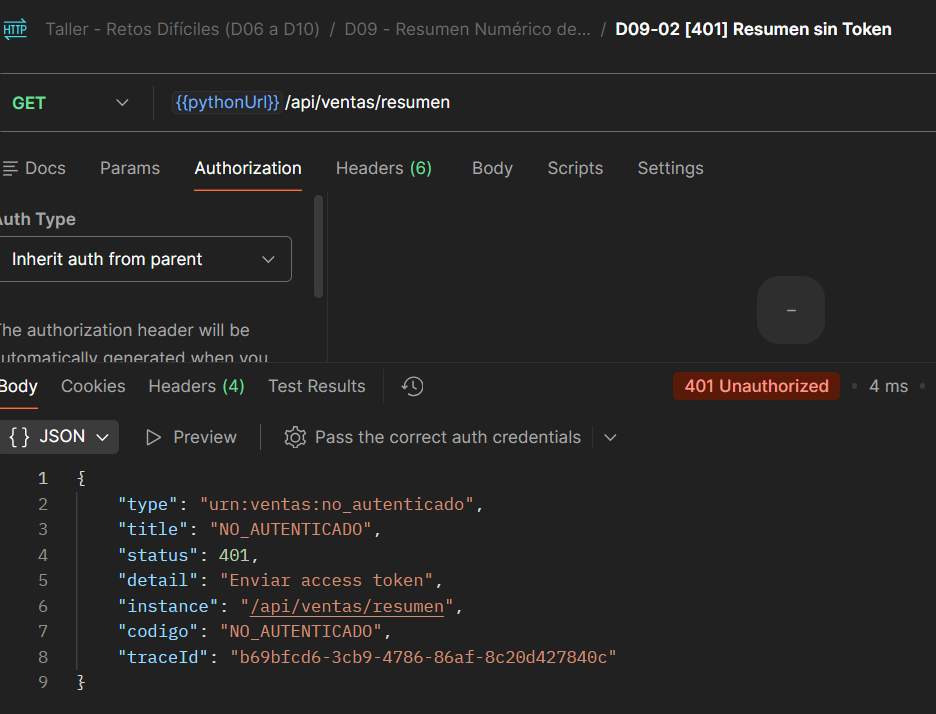
\includegraphics[width=0.95\textwidth]{imagenes/media/image30.png}
    \caption{D09-02: Rechazo de resumen sin token de autorización (401 Unauthorized).}
    \label{fig:d09_02}
\end{figure}

\subsubsection{5. Persistencia (MySQL)}
\begin{lstlisting}[language=SQL]
SELECT 
    COUNT(*) AS total_ventas,
    SUM(CASE WHEN estado = 'COMPLETADA' THEN 1 ELSE 0 END) AS completadas,
    SUM(CASE WHEN estado = 'FALLIDA' THEN 1 ELSE 0 END) AS fallidas,
    SUM(CASE WHEN estado = 'COMPLETADA' THEN precio_acordado ELSE 0 END) AS total_ingresos
FROM ventas WHERE usuario = 'admin-local';
\end{lstlisting}

\begin{figure}[H]
    \centering
    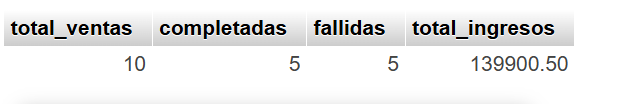
\includegraphics[width=0.95\textwidth]{imagenes/media/sql_d09.png}
    \caption{Evidencia SQL en MySQL: Agregación real de ventas con total de ingresos \$139900.50 y conteos exactos.}
    \label{fig:sql_d09}
\end{figure}

\subsubsection{6. Explicación}
El valor devuelto por la API (\texttt{"totalIngresos": "139900.50"}, 5 completadas, 5 fallidas) coincide al centavo con la consulta de agregación directa en MySQL, demostrando que los montos de ventas fallidas fueron excluidos.

\newpage
% ----------------------------------------------------------------------------
% D10
% ----------------------------------------------------------------------------
\subsection{D10 | Emitir comprobante JSON de una venta confirmada}
\textbf{Servicio y contrato:} FastAPI $\cdot$ \texttt{GET /api/ventas/\{id\}/comprobante}

\subsubsection{1. Diagnóstico}
Una vez concluida satisfactoriamente la venta de un vehículo con confirmación remota en Java, el comprador y el vendedor carecían de un comprobante digital unificado que agrupara la información del vehículo, del comprador y el precio pactado definitivo.

\subsubsection{2. Diseño}
Se implementó el endpoint \texttt{GET /api/ventas/\{id\}/comprobante}. Reglas de negocio:
\begin{itemize}
    \item Existencia y Autorización: Retornar \texttt{404} si la venta no existe y \texttt{403} si no pertenece al usuario autenticado.
    \item Condición de Estado: El comprobante solo puede emitirse si la venta se encuentra en estado \texttt{COMPLETADA}. Si la venta está \texttt{FALLIDA} o \texttt{PENDIENTE}, debe responder \texttt{409 Conflict} con código \texttt{VENTA\_NO\_COMPLETADA}.
    \item Integridad del Precio: El comprobante toma obligatoriamente el \texttt{precio\_acordado} guardado en la venta al momento de confirmar, garantizando inmutabilidad histórica frente a futuros cambios en el catálogo de vehículos.
\end{itemize}

\subsubsection{3. Implementación}
\begin{lstlisting}[language=Python]
@router.get("/ventas/{id}/comprobante")
def comprobante_venta(id: int, u=Depends(identidad)):
    vendedor(u)
    with SessionLocal() as db:
        v = db.get(Venta, id)
        if v is None:
            raise ApiError(404, "VENTA_NO_EXISTE", "Venta inexistente")
        propietario(u, v.usuario)
        if v.estado != "COMPLETADA":
            raise ApiError(409, "VENTA_NO_COMPLETADA", f"No se puede emitir comprobante para estado {v.estado}")
        return {
            "idVenta": v.id, "operacionId": v.operacion_id, "fecha": v.fecha.isoformat() + "Z",
            "comprador": {
                "id": v.comprador.id, "documento": v.comprador.documento,
                "nombre": v.comprador.nombre, "correo": v.comprador.correo
            },
            "vehiculoId": v.vehiculo_id,
            "precioConfirmado": str(v.precio_acordado), "moneda": v.moneda, "estado": v.estado
        }
\end{lstlisting}

\subsubsection{4. Validación}
\begin{table}[H]
\centering
\small
\begin{tabularx}{\textwidth}{l p{4.5cm} p{2cm} c c X}
\toprule
\textbf{ID} & \textbf{Método / URL} & \textbf{Estado Venta} & \textbf{HTTP Esp.} & \textbf{HTTP Obt.} & \textbf{Resultado} \\
\midrule
D10-01 & \texttt{GET /api/ventas/3/comprobante} & COMPLETADA & 200 & 200 & Comprobante generado con comprador y precio pactado. \\
D10-02 & \texttt{GET /api/ventas/1/comprobante} & FALLIDA & 409 & 409 & Conflicto de negocio \texttt{VENTA\_NO\_COMPLETADA}. \\
D10-03 & \texttt{GET /api/ventas/99999/comprobante} & Inexistente & 404 & 404 & Rechazo \texttt{VENTA\_NO\_EXISTE}. \\
\bottomrule
\end{tabularx}
\caption{Matriz de pruebas del reto D10.}
\end{table}

\begin{figure}[H]
    \centering
    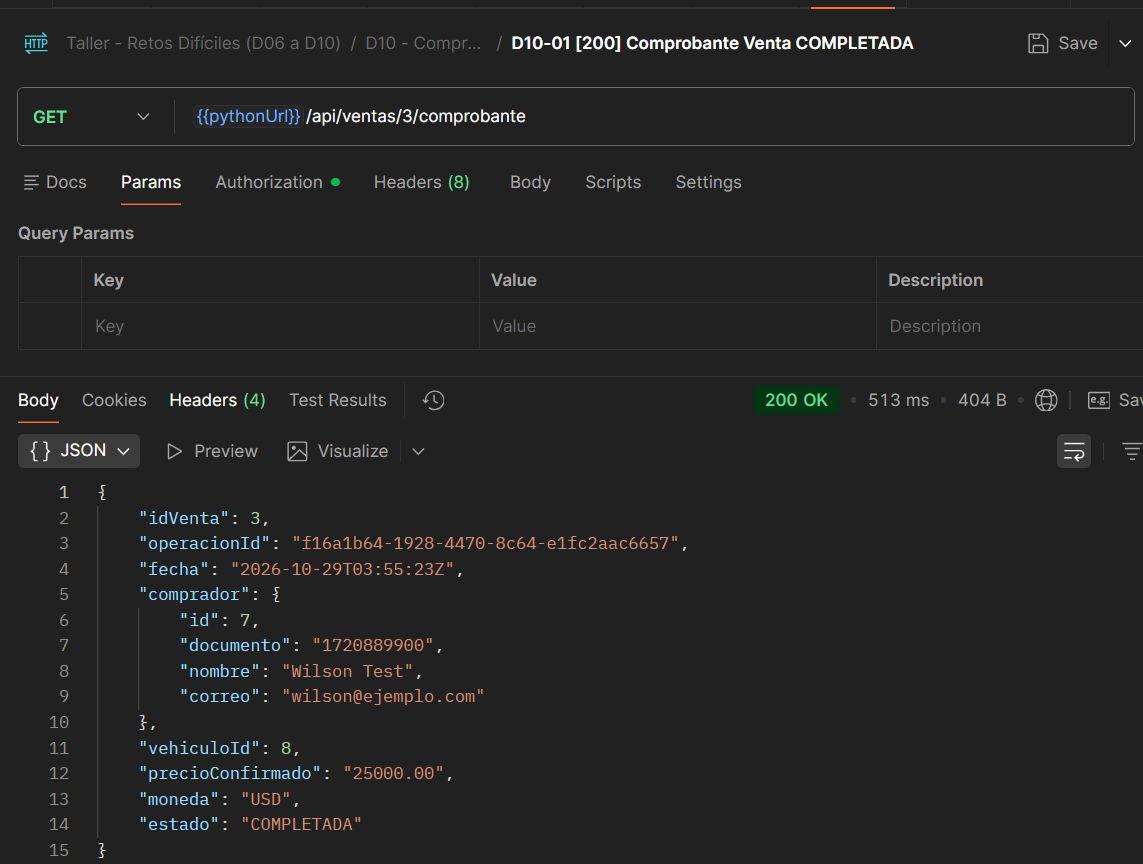
\includegraphics[width=0.95\textwidth]{imagenes/media/image31.png}
    \caption{D10-01: Comprobante JSON para venta COMPLETADA (200 OK).}
    \label{fig:d10_01}
\end{figure}

\begin{figure}[H]
    \centering
    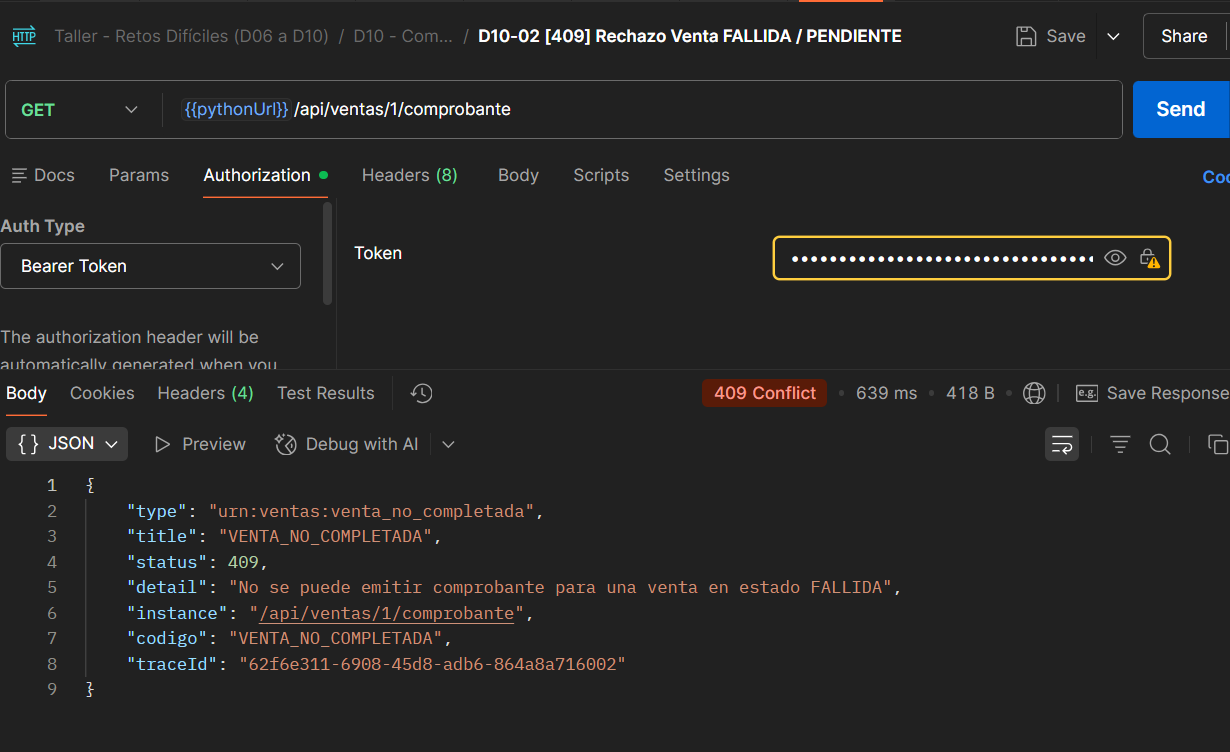
\includegraphics[width=0.95\textwidth]{imagenes/media/image32.png}
    \caption{D10-02: Rechazo para venta en estado FALLIDA (409 Conflict).}
    \label{fig:d10_02}
\end{figure}

\begin{figure}[H]
    \centering
    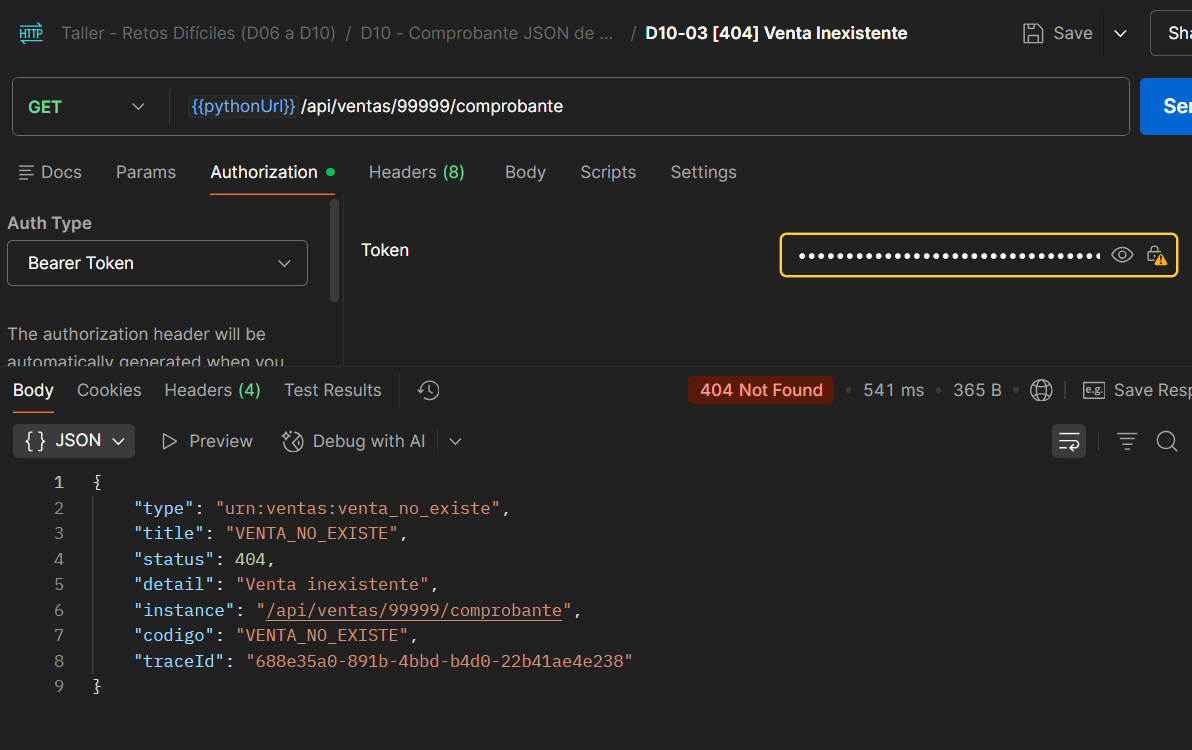
\includegraphics[width=0.95\textwidth]{imagenes/media/image33.png}
    \caption{D10-03: Rechazo por venta inexistente (404 Not Found).}
    \label{fig:d10_03}
\end{figure}

\subsubsection{5. Persistencia (MySQL)}
\begin{lstlisting}[language=SQL]
SELECT v.id, v.operacion_id, v.precio_acordado, v.moneda, v.estado, v.fecha, c.nombre, c.documento
FROM ventas v INNER JOIN compradores c ON v.comprador_id = c.id WHERE v.id = 3;
\end{lstlisting}

\begin{figure}[H]
    \centering
    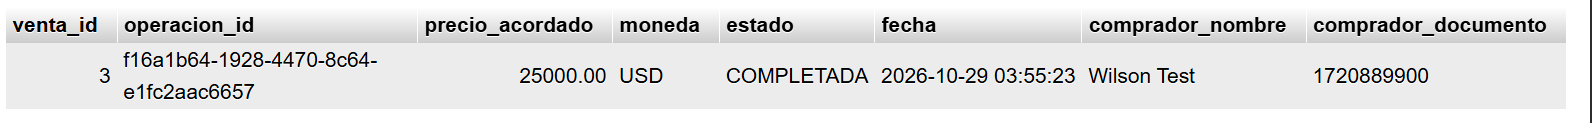
\includegraphics[width=0.95\textwidth]{imagenes/media/sql_d10.png}
    \caption{Evidencia SQL en MySQL: Registro relacional de la venta 3 vinculada con su comprador y precio confirmado 25000.00 USD.}
    \label{fig:sql_d10}
\end{figure}

\subsubsection{6. Explicación}
La relación directa entre las entidades relacionales \texttt{Venta} y \texttt{Comprador} mediante clave foránea permite la hidratación eficiente del comprobante en una sola lectura sin requerir consultas manuales adicionales en la base de datos.

\newpage

% ============================================================================
% GUÍA DE EVIDENCIAS SQL REALES
% ============================================================================
\section{Guía de Obtención de Evidencias SQL en MySQL}

Para documentar las capturas de base de datos exigidas por la rúbrica del informe sin alterar los datos reales, se debe abrir \textbf{phpMyAdmin} (\texttt{http://localhost/phpmyadmin}) o la consola de MySQL en XAMPP y ejecutar las siguientes sentencias sobre la base \texttt{venta\_vehiculos}:

\begin{enumerate}
    \item \textbf{Para Retos F01 y D07 (Compradores y Búsqueda):}
\begin{lstlisting}[language=SQL]
SELECT id, documento, nombre, correo, usuario FROM compradores WHERE usuario = 'admin-local';
\end{lstlisting}
    \textit{Captura sugerida:} Tomar captura de la cuadrícula de resultados donde se visualice la lista de compradores asociados a \texttt{admin-local}.

    \item \textbf{Para Retos F02 y D08 (Consulta y Actualización Inmutable):}
\begin{lstlisting}[language=SQL]
SELECT id, documento, nombre, correo, usuario FROM compradores WHERE id = 1;
\end{lstlisting}
    \textit{Captura sugerida:} Demuestra que \texttt{nombre} es \texttt{"Pedro Actualizado"} y que el \texttt{documento} permanece como \texttt{"12345678"}.

    \item \textbf{Para Retos F03 y D06 (Orden y Paginación de Ventas):}
\begin{lstlisting}[language=SQL]
SELECT id, operacion_id, vehiculo_id, comprador_id, estado, precio_acordado, fecha 
FROM ventas WHERE usuario = 'admin-local' ORDER BY fecha DESC, id DESC LIMIT 2 OFFSET 0;
\end{lstlisting}
    \textit{Captura sugerida:} Muestra las dos primeras ventas ordenadas coincidentes con la página 1 de Postman.

    \item \textbf{Para Reto F04 (Filtro por Estado):}
\begin{lstlisting}[language=SQL]
SELECT id, operacion_id, vehiculo_id, estado, precio_acordado 
FROM ventas WHERE usuario = 'admin-local' AND estado = 'COMPLETADA';
\end{lstlisting}
    \textit{Captura sugerida:} Evidencia que solo se devuelven ventas en estado \texttt{COMPLETADA}.

    \item \textbf{Para Reto F05 (Filtro de Vehículos en Java):}
\begin{lstlisting}[language=SQL]
SELECT id_vehiculo, marca, modelo, estado, precio FROM vehiculos WHERE marca = 'Toyota' AND estado = 'DISPONIBLE';
\end{lstlisting}
    \textit{Captura sugerida:} Cuadrícula con los vehículos que cumplen ambos criterios.

    \item \textbf{Para Reto D09 (Métricas Numéricas):}
\begin{lstlisting}[language=SQL]
SELECT 
    COUNT(*) AS total_ventas,
    SUM(CASE WHEN estado = 'COMPLETADA' THEN 1 ELSE 0 END) AS completadas,
    SUM(CASE WHEN estado = 'FALLIDA' THEN 1 ELSE 0 END) AS fallidas,
    SUM(CASE WHEN estado = 'COMPLETADA' THEN precio_acordado ELSE 0 END) AS total_ingresos
FROM ventas WHERE usuario = 'admin-local';
\end{lstlisting}
    \textit{Captura sugerida:} Fila única con el total de ingresos \texttt{139900.50} y conteos exactos.

    \item \textbf{Para Reto D10 (Comprobante Confirmado):}
\begin{lstlisting}[language=SQL]
SELECT v.id, v.operacion_id, v.precio_acordado, v.moneda, v.estado, c.nombre, c.documento
FROM ventas v INNER JOIN compradores c ON v.comprador_id = c.id WHERE v.id = 3;
\end{lstlisting}
    \textit{Captura sugerida:} Registro de la venta completada vinculada a su comprador.
\end{enumerate}

\newpage

% ============================================================================
% CONCLUSIONES Y LECCIONES APRENDIDAS
% ============================================================================
\section{Conclusiones y Lecciones Aprendidas}

\begin{itemize}
    \item \textbf{Separación Estricta de Capas:} La implementación de los retos F01 a D10 evidenció la importancia de mantener la separación de responsabilidades: los Routers gestionan el protocolo HTTP y la seguridad, los Servicios aplican la lógica de negocio y los Repositorios optimizan el acceso a la base de datos.
    \item \textbf{Prevención de Colisiones de Enrutamiento:} Se aprendió que en frameworks como FastAPI, las rutas estáticas (\texttt{/ventas/resumen}) deben declararse antes de las rutas parametrizadas (\texttt{/ventas/\{id\}}), evitando fallos de parseo.
    \item \textbf{Seguridad y Aislamiento Multi-Inquilino:} El filtrado a nivel de repositorio vinculado al token JWT garantizó que ningún usuario acceda a datos ajenos, mientras que el uso de parámetros tipados de SQLAlchemy neutralizó intentos de inyección SQL.
    \item \textbf{Precisión Numérica:} El manejo de tipos \texttt{Decimal} previno inconsistencias de redondeo en importes monetarios, asegurando que los cálculos reportados coincidan de forma exacta con la base de datos relacional.
    \item \textbf{Dificultades Superadas:} La principal dificultad consistió en coordinar el ciclo de vida de dos pilas tecnológicas diferentes (Java Spring Boot y Python FastAPI) compartiendo la misma base relacional, lo cual se resolvió manteniendo esquemas compatibles y contratos HTTP homogéneos conformes a los estándares RFC.
\end{itemize}

\end{document}
